% =====================================================================
%  Manual del visor del Catastro + registro de cambios a los datos
%
%  Se compila con Tectonic (XeTeX):
%     tectonic -X compile visor_catastro.tex
%
%  Todas las cifras de este documento salen de fuentes comprobadas:
%  frontend/public/datos/manifest.json, el codigo del ETL y el propio
%  sitio publicado. Ninguna esta escrita de memoria.
% =====================================================================
\documentclass[11pt,a4paper]{report}

\usepackage{fontspec}
\usepackage[spanish,es-tabla,es-noquoting,es-nolists]{babel}
\usepackage[margin=2.6cm,top=3cm,bottom=2.8cm]{geometry}
\usepackage{booktabs}
\usepackage{longtable}
\usepackage{array}
\usepackage[table]{xcolor}
\usepackage{graphicx}
\usepackage{fancyhdr}
\usepackage{enumitem}
\usepackage{titlesec}
\usepackage{tcolorbox}
\usepackage{caption}
\usepackage{float}
\usepackage{placeins}
\usepackage{hyperref}

% Sin esto, las figuras de pantalla completa dejan paginas medio vacias: por
% defecto LaTeX no admite mas de un 70 % de figura en una pagina con texto.
\renewcommand{\topfraction}{0.92}
\renewcommand{\bottomfraction}{0.85}
\renewcommand{\textfraction}{0.06}
\renewcommand{\floatpagefraction}{0.75}
\setcounter{topnumber}{3}
\setcounter{totalnumber}{4}

% Calibri y Consolas estan en el equipo; Open Sans (la institucional) solo
% existe como fuente variable, que XeTeX no sabe instanciar.
\setmainfont{Calibri}
\setmonofont{Consolas}[Scale=0.88]

% Verde institucional tomado del propio visor (frontend/src/index.css: #064928).
\definecolor{conaf}{HTML}{064928}
\definecolor{conafclaro}{HTML}{E7EFE9}
\definecolor{aviso}{HTML}{8A5A00}
\definecolor{grisfino}{HTML}{6F7A73}
\definecolor{filagris}{HTML}{F2F3F0}

\hypersetup{colorlinks=true, linkcolor=conaf, urlcolor=conaf, citecolor=conaf,
  pdftitle={Visor del Catastro de Usos de la Tierra y Recursos Vegetacionales},
  pdfauthor={CONAF - Unidad de Informacion y Analisis},
  pdfsubject={Manual de uso y registro de cambios aplicados a los datos}}

\tcbuselibrary{skins,breakable}
\newtcolorbox{nota}[1][]{breakable, colback=conafclaro, colframe=conaf,
  boxrule=0.4pt, left=7pt, right=7pt, top=6pt, bottom=6pt, #1}
\newtcolorbox{alerta}[1][]{breakable, colback=yellow!8, colframe=aviso,
  boxrule=0.7pt, left=7pt, right=7pt, top=6pt, bottom=6pt, #1}

\titleformat{\part}[display]
  {\normalfont\centering\color{conaf}}{\Large\bfseries\partname\ \thepart}{14pt}{\Huge\bfseries}
\titleformat{\chapter}[display]
  {\normalfont\huge\bfseries\color{conaf}}{\large\chaptertitlename\ \thechapter}{6pt}{\Huge}
\titlespacing*{\chapter}{0pt}{-10pt}{24pt}
\titleformat{\section}{\normalfont\Large\bfseries\color{conaf}}{\thesection}{0.8em}{}
\titleformat{\subsection}{\normalfont\large\bfseries}{\thesubsection}{0.8em}{}

\pagestyle{fancy}
\fancyhf{}
\fancyhead[L]{\footnotesize\color{grisfino}Visor del Catastro · CONAF}
\fancyhead[R]{\footnotesize\color{grisfino}\nouppercase{\leftmark}}
\fancyfoot[C]{\small\thepage}
\renewcommand{\headrulewidth}{0.3pt}

\captionsetup{font=small, labelfont={bf,color=conaf}}
\setlength{\parskip}{0.5em}
\setlength{\parindent}{0pt}
\setlist{itemsep=2pt, topsep=4pt, parsep=0pt}

% Columna de parrafo alineada a la izquierda: sin esto las tablas anchas
% abren huecos enormes entre palabras.
\newcolumntype{L}[1]{>{\raggedright\arraybackslash}p{#1}}
\newcommand{\campo}[1]{\textcolor{conaf}{\textbf{#1}}}
\newcommand{\orig}[1]{\texttt{\small #1}}

\begin{document}

% ---------------------------------------------------------------- portada
\begin{titlepage}
\thispagestyle{empty}
\noindent
\includegraphics[width=\textwidth]{img/banner.png}
\vspace{1.6cm}

{\color{conaf}\Huge\bfseries Visor del Catastro de Usos\\[2mm]
de la Tierra y Recursos Vegetacionales\par}
\vspace{7mm}
{\Large Manual de uso y registro de los cambios\\[1mm] aplicados a los datos\par}
\vspace{6mm}
{\color{grisfino}\large Corporación Nacional Forestal\\
Gerencia de Fiscalización Forestal y Evaluación Ambiental\\
Unidad de Información y Análisis\par}

\vfill
\noindent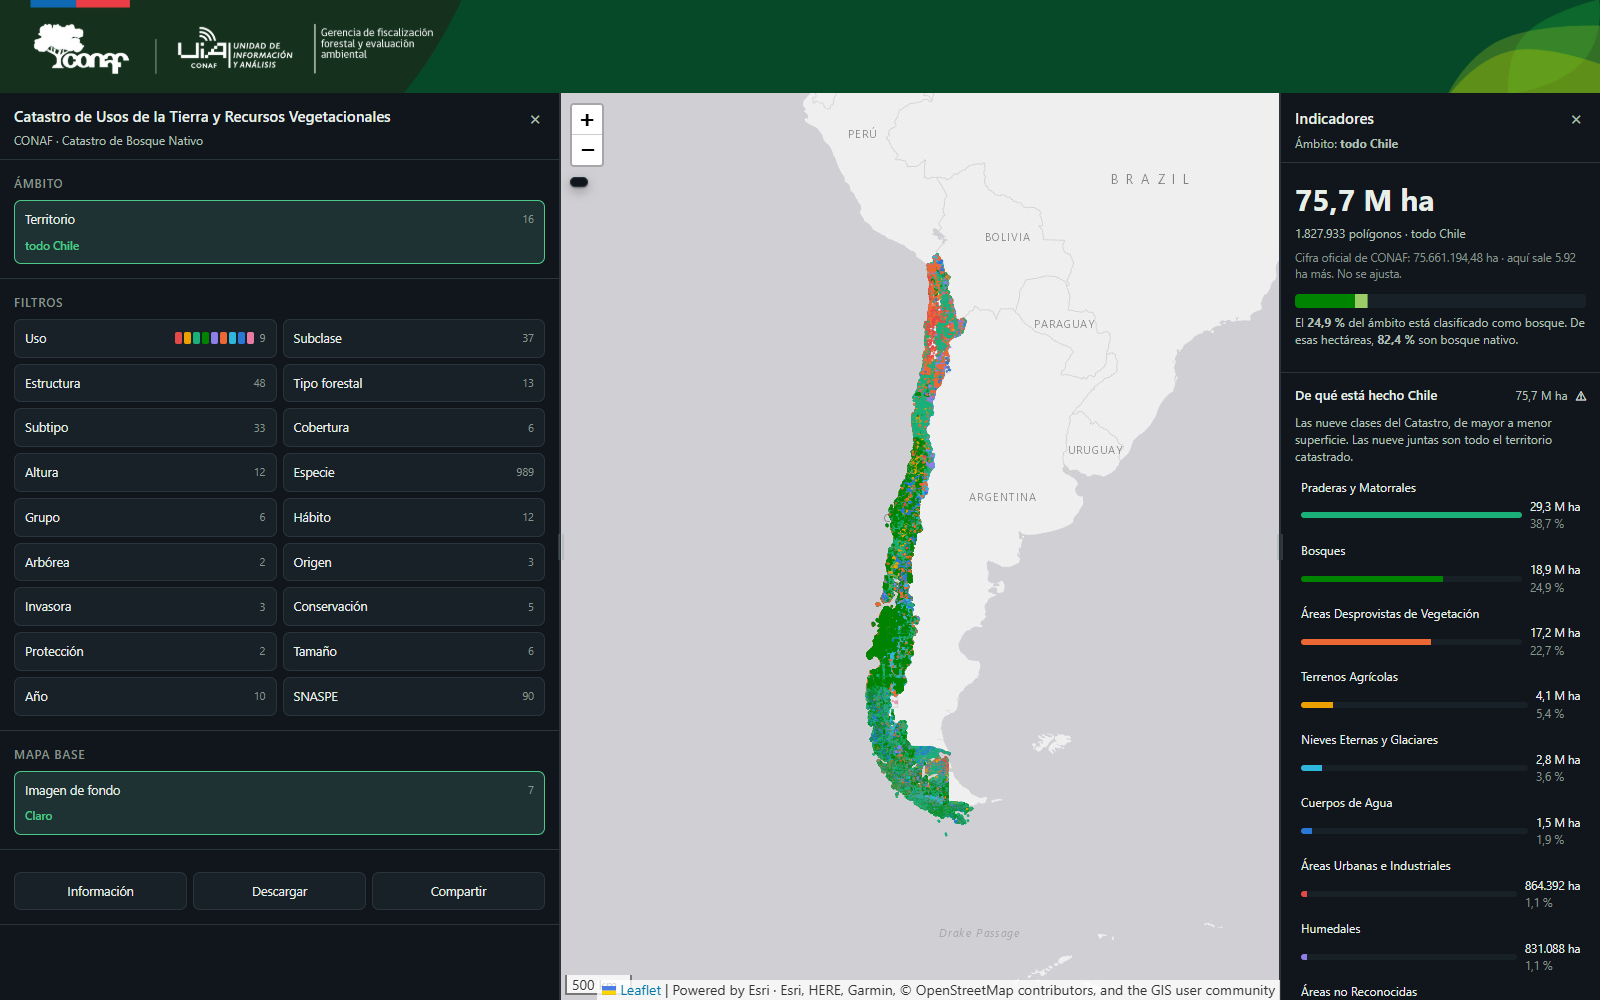
\includegraphics[width=\textwidth]{img/visor-completo.png}
\vfill

{\small\color{grisfino}22 de septiembre de 2026\\
\url{https://sud-austral.github.io/coipo_vista_catastro/}\par}
\end{titlepage}

% ---------------------------------------------------------------- índice
\pagenumbering{roman}
\tableofcontents
\cleardoublepage
\pagenumbering{arabic}

% ================================================================
\part{Manual: qué es el visor, cómo se usa y qué muestra}
% ================================================================

\chapter{Qué es este visor}

\section{En una frase}

Es un mapa público de todo el Catastro de Usos de la Tierra y Recursos
Vegetacionales de CONAF: \textbf{1.827.933 polígonos} que suman
\textbf{75.661.200,40 hectáreas}, con veinte controles para acotar lo que se
mira y un panel que recalcula las cifras cada vez que se cambia algo.

Se abre en un navegador, en la dirección

\begin{center}
\large\url{https://sud-austral.github.io/coipo_vista_catastro/}
\end{center}

No hay que instalar nada, no hay que pedir una cuenta y no hay clave. Funciona
en Chrome, Edge o Firefox actualizados.

\section{Para qué sirve, en concreto}

\begin{itemize}
  \item \campo{Consultar} cuánta superficie de una clase hay en una región, una
        provincia o una comuna, sin pedirle una consulta a nadie.
  \item \campo{Ubicar} dónde están los polígonos de una especie, un tipo
        forestal o una estructura determinada.
  \item \campo{Cruzar} condiciones: por ejemplo, renoval de roble dentro del
        SNASPE en la Región de Los Ríos.
  \item \campo{Llevarse} el resultado: un reporte en PDF, las cifras en CSV o
        los propios polígonos en CSV o GeoJSON.
  \item \campo{Compartir} una consulta exacta mediante un enlace que reproduce
        la misma vista en la pantalla de otra persona.
\end{itemize}

\section{Qué NO es}

Esto importa tanto como lo anterior, porque casi todos los malentendidos con
este visor nacen aquí.

\begin{alerta}
\begin{itemize}[leftmargin=*]
  \item \campo{No es un registro de propiedad.} El Catastro no anota de quién es
        un terreno. Ningún polígono corresponde a un predio ni a un rol de
        avalúo, y el visor no puede decir de quién es nada.
  \item \campo{No califica el estado de un bosque.} Describe cobertura y
        estructura; no dice si está sano, degradado o bien manejado.
  \item \campo{No mide cambio en el tiempo.} Cada región se catastró en un año
        distinto y no hay dos levantamientos comparables de la misma región.
        Restar una región de otra no mide ningún cambio: compara dos años.
  \item \campo{No sustituye una inspección en terreno} ni un informe de
        fiscalización. La unidad mínima cartografiable deja fuera los rodales
        pequeños.
  \item \campo{No dice si una especie está amenazada.} El Catastro no registra
        estado de conservación; véase el aviso de la página
        \pageref{sec:conservacion}.
\end{itemize}
\end{alerta}

\section{De dónde salen los datos y cuánto pesan}

El visor no consulta ninguna base de datos mientras se usa: al abrirlo descarga
de una vez el archivo de datos, de \textbf{49.354.191 bytes} (47,1~MiB), con los
1.827.933 puntos ya preparados, más el catálogo \orig{manifest.json} del que
salen todos los vocabularios y las cifras del panel. A partir de ahí todo el
filtrado ocurre en el
propio computador. Por eso responde al instante al mover un filtro, y por eso la
primera carga tarda unos segundos, los que la conexión de cada oficina tarde en
traer ese archivo.

Por la red viajan unos \textbf{19,5~MiB}, porque el servidor entrega los
archivos comprimidos.

\begin{nota}
\campo{Consecuencia práctica.} Una vez cargado, el visor funciona aunque la
conexión se ponga lenta. Lo único que sigue necesitando red es el mapa de fondo
(las imágenes de satélite o de calles), que viene de servidores externos.
\end{nota}

\section{En pantallas chicas}

La disposición cambia en dos puntos. Por debajo de \textbf{1200~px} de ancho los
paneles se estrechan; por debajo de \textbf{900~px} —una tableta en vertical o
un teléfono— los dos paneles dejan de ocupar sitio y pasan a ser cajones que se
abren y se cierran: el mapa ocupa toda la pantalla, con un botón de menú arriba
a la izquierda para los controles y otro arriba a la derecha para los
indicadores.

\begin{nota}
\campo{El visor recuerda cómo dejaste los paneles} —su ancho y si estaban
plegados— para la próxima visita desde ese mismo navegador. Los filtros no: ésos
viajan en la dirección web, que es lo que se comparte.
\end{nota}

% ----------------------------------------------------------------
\chapter{La pantalla, zona por zona}

Al entrar, la pantalla se divide en cuatro zonas.

\begin{figure}[htbp]
\centering
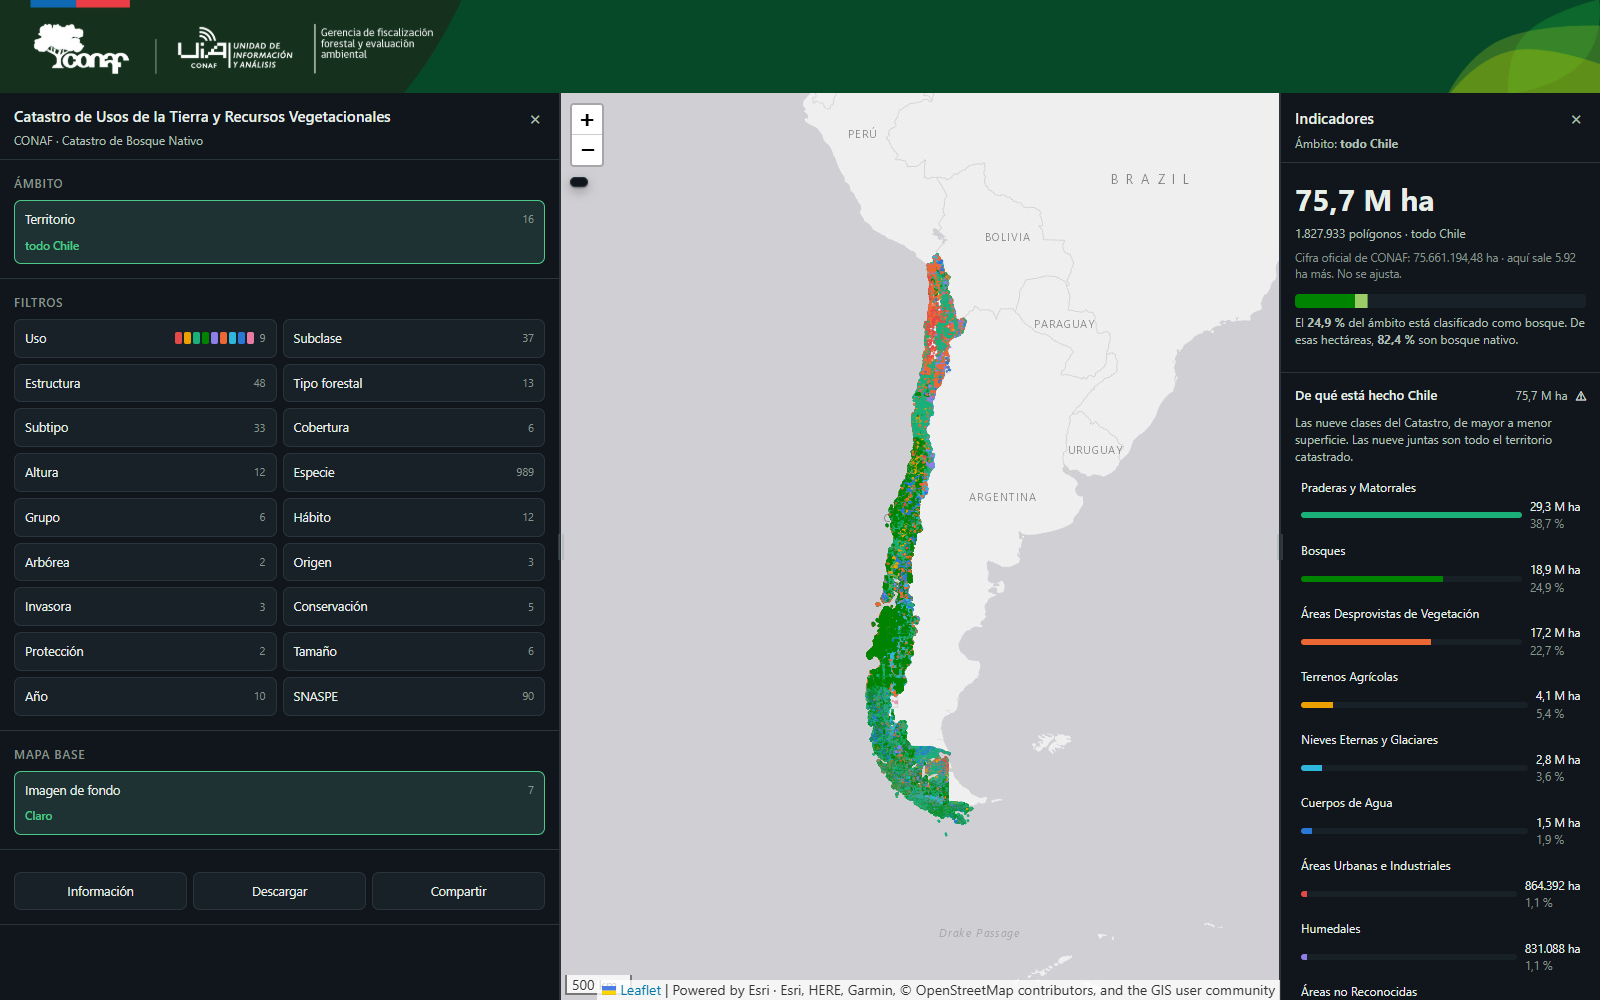
\includegraphics[width=\textwidth]{img/visor-completo.png}
\caption{Pantalla completa del visor recién abierto: encabezado institucional
arriba, panel de control a la izquierda, mapa al centro y panel de indicadores
a la derecha.}
\end{figure}

\section{El encabezado institucional}
Arriba, la franja verde con los logotipos de CONAF y de la Unidad de Información
y Análisis, y la mención a la Gerencia de Fiscalización Forestal y Evaluación
Ambiental. Es fijo: no tiene controles.

\section{El panel de control, a la izquierda}
Contiene todo lo que se puede elegir, en tres bloques —\campo{ÁMBITO},
\campo{FILTROS} y \campo{MAPA BASE}— y tres botones de acción al pie:
\campo{Información}, \campo{Descargar} y \campo{Compartir}.

\begin{figure}[htbp]
\centering
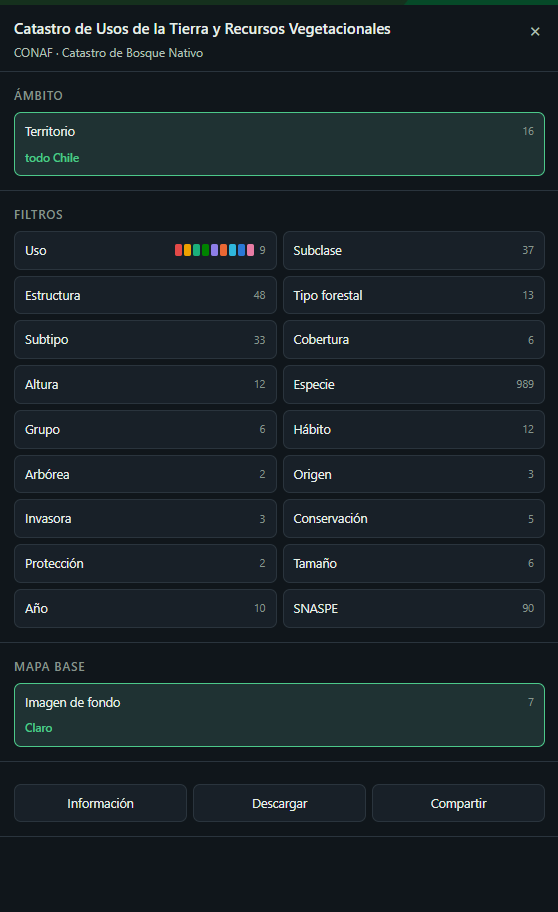
\includegraphics[width=0.52\textwidth]{img/panel-controles.png}
\caption{El panel de control. El número pequeño a la derecha de cada botón es
la cantidad de categorías disponibles en ese filtro.}
\end{figure}

Se puede plegar con la \texttt{×} de su esquina, para dejarle la pantalla
entera al mapa; entonces aparece en su lugar un botón de tres rayas para volver
a abrirlo.

\section{El mapa, al centro}
Muestra un punto por polígono. Trae los botones \texttt{+} y \texttt{−} para
acercar y alejar, la etiqueta con la fecha de la imagen de fondo cuando
corresponde, una escala gráfica y, abajo, la atribución obligatoria del mapa de
fondo.

\begin{nota}
\campo{El visor tiene tema claro y oscuro, pero no un botón para cambiarlo.}
Sigue el que tenga configurado el sistema operativo. Para verlo en oscuro hay
que cambiar el tema de Windows, no el del visor.
\end{nota}

\section{El panel de indicadores, a la derecha}
Es la parte que más gente pasa por alto y la que más rinde: recalcula todas las
cifras cada vez que se toca un filtro. Se detalla en el capítulo~\ref{cap:indicadores}.

\section{Lo primero que se ve: la pantalla de carga}

Antes del mapa aparece una pantalla con la banda institucional ya dibujada y el
texto \campo{«Cargando el Catastro nacional…»}. Si la descarga se alarga, a los
quince segundos añade una segunda línea: \campo{«Está tardando más de lo
normal»}.

\begin{nota}
\campo{Ese segundo mensaje no significa que algo se haya roto:} significa que la
conexión está tardando. Conviene esperar. Mientras el mapa termina de bajar, el
panel de indicadores de la derecha \campo{ya muestra las cifras nacionales},
porque su catálogo llega antes que los puntos.
\end{nota}

\section{El cartel de la primera visita}
La primera vez aparece un cartel sobre el mapa con la advertencia más importante
de todas:

\begin{nota}
«Cada punto es el centroide de un polígono del Catastro, no una parcela ni un
predio. Su posición representa al polígono completo; la superficie real está en
el atributo.»
\end{nota}

Se cierra con \campo{Entendido} y no vuelve a salir.

% ----------------------------------------------------------------
\chapter{Cómo se filtra}
\label{cap:filtros}

\section{El principio, en dos líneas}

Todos los controles se \campo{cruzan entre sí}: el mapa y todas las cifras
muestran sólo los polígonos que cumplen \emph{todas} las condiciones a la vez.
Un filtro que no se toca no restringe nada.

\section{El ámbito territorial}

El bloque \campo{ÁMBITO} tiene un solo control, \campo{Territorio}, y es
distinto de los demás: en vez de marcar varias casillas se elige \emph{un}
ámbito —todo Chile, una región, una provincia o una comuna— y el visor recorta
el mapa y todas las cifras a ese territorio.

\begin{figure}[htbp]
\centering
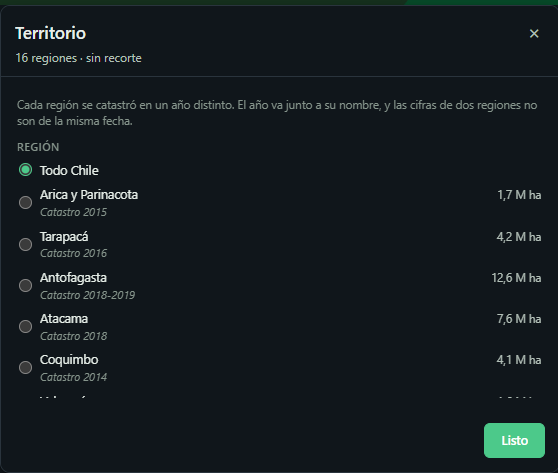
\includegraphics[width=0.52\textwidth]{img/modal-territorio.png}
\caption{Selector de territorio. Junto a cada región va el año en que se
catastró y su superficie.}
\end{figure}

\begin{alerta}
\campo{No todas las regiones son del mismo año.} El selector lo dice junto a
cada nombre: Coquimbo es catastro 2014, Arica y Parinacota 2015, Antofagasta
2018--2019. Sobre dieciséis regiones hay diez fechas distintas, entre 2014 y
2024. Comparar dos regiones puede ser comparar dos fotos tomadas en años
distintos.
\end{alerta}

\section{Los dieciocho filtros}

El bloque \campo{FILTROS} tiene dieciocho controles. Cada uno abre una lista de
casillas; se marcan las que interesan y se pulsa \campo{Listo}.

\begin{longtable}{@{}L{3.2cm}r L{8.6cm}@{}}
\toprule
\textbf{Filtro} & \textbf{Categorías} & \textbf{Qué selecciona}\\
\midrule
\endfirsthead
\toprule
\textbf{Filtro} & \textbf{Categorías} & \textbf{Qué selecciona}\\
\midrule
\endhead
\campo{Uso} & 9 & La clase de uso de la tierra: Bosques, Praderas y Matorrales, Terrenos Agrícolas, etc. Es la variable que da color al mapa.\\
\campo{Subclase} & 37 & El subuso dentro de la clase: por ejemplo, dentro de Bosques, «Bosque Nativo», «Plantación» o «Bosque Mixto».\\
\campo{Estructura} & 48 & La estructura de la vegetación: Adulto, Renoval, Adulto-Renoval, Achaparrado, Estepa Patagónica, etc.\\
\campo{Tipo forestal} & 13 & Los doce tipos forestales de la Ley —Alerce, Araucaria, Lenga, Roble-Raulí-Coihue, Esclerófilo…— más «No Aplica» para el territorio que no es bosque nativo (60,1~M ha).\\
\campo{Subtipo} & 33 & El subtipo dentro del tipo forestal.\\
\campo{Cobertura} & 6 & Densidad del dosel: Denso, Semidenso, Abierto, Muy Abierto, Escaso, y «No Aplica» donde la pregunta no tiene sentido (36,7~M ha: agua, glaciares, zonas urbanas).\\
\campo{Altura} & 12 & Altura del dosel, en tramos de metros.\\
\campo{Especie} & 989 & La especie dominante del polígono.\\
\campo{Grupo} & 6 & Grupo botánico de esa especie: Latifoliada, Conifera, Monocotiledonea, Helecho, Briofita, Gimnosperma.\\
\campo{Hábito} & 12 & Forma de crecimiento: Arbol, Arbusto, Graminea, Acuatica, Hierba, Suculenta, Cactacea, Bambu, Briofita, Helecho, Trepadora, Palma.\\
\campo{Arbórea} & 2 & Si la especie dominante es arbórea o no.\\
\campo{Origen} & 3 & Nativa, Exotica o Sin determinar.\\
\campo{Invasora} & 3 & Si la especie está clasificada como invasora.\\
\campo{Conservación} & 5 & Categoría de amenaza de la especie. \textbf{Léase antes el aviso de la sección~\ref{sec:conservacion}.}\\
\campo{Protección} & 2 & Dentro o fuera del SNASPE.\\
\campo{Tamaño} & 6 & Tamaño del polígono, en tramos: menos de 1~ha, 1--5, 5--20, 20--100, 100--500, 500 o más.\\
\campo{Año} & 10 & Año del levantamiento (2014 a 2024, algunos en rangos).\\
\campo{SNASPE} & 90 & Unidad concreta del Sistema Nacional de Áreas Silvestres Protegidas del Estado.\\
\bottomrule
\caption{Los dieciocho filtros, con el número de categorías que ofrece cada uno.}
\end{longtable}

\begin{alerta}
\campo{En el filtro de Especie hay nombres que aparecen repetidos, y no es un
error.} La lista muestra el nombre común, y 48 de esos nombres corresponden a
más de una especie: «quisco» sale doce veces, «coirón» ocho, «eucalipto» siete.
En total afecta a 137 de las 989 especies. Son especies distintas con el mismo
nombre vulgar; para distinguirlas hay que mirar el nombre científico, que
aparece en la ficha del punto.
\end{alerta}

\begin{alerta}
\campo{Las etiquetas de los seis últimos filtros van sin tilde.} «Conifera»,
«Monocotiledonea», «Arbol», «Bambu», «Cactacea», «Acuatica», «Graminea» y
«Exotica» se publican tal como vienen de la tabla auxiliar de especies. No es
un descuido del manual: es lo que muestra el filtro, y buscarlas con tilde no
las encuentra.
\end{alerta}

\begin{nota}
\campo{El número no es el del catálogo, es el de lo que hay.} El visor lista
sólo las categorías que tienen al menos un polígono. El catálogo de subclases
tiene 43 entradas y el filtro muestra 37; el de estructuras tiene 58 y el
filtro muestra 48. Las que faltan son categorías oficiales sin ningún polígono
en los datos publicados.
\end{nota}

\section{Cómo se ve un filtro por dentro}

\begin{figure}[htbp]
\centering
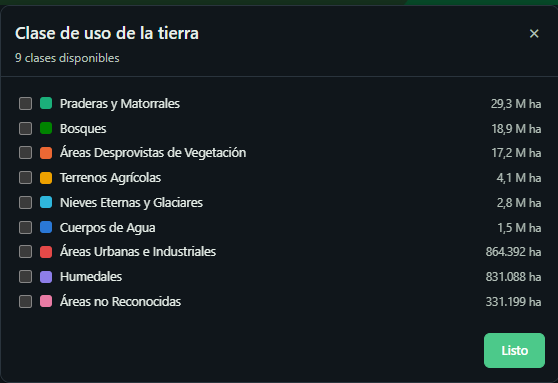
\includegraphics[width=0.52\textwidth]{img/modal-uso.png}
\caption{El filtro \emph{Uso} abierto. Cada línea trae su color en el mapa y la
superficie que representa, ordenadas de mayor a menor.}
\end{figure}

Al marcar una casilla, el mapa y las cifras se rehacen al momento. En la
cabecera del filtro se lee cuántas categorías hay elegidas —«1 de 9 clases
elegidas»— y abajo a la izquierda aparece \campo{Quitar el filtro de uso}, que
lo deja como estaba.

\begin{figure}[htbp]
\centering
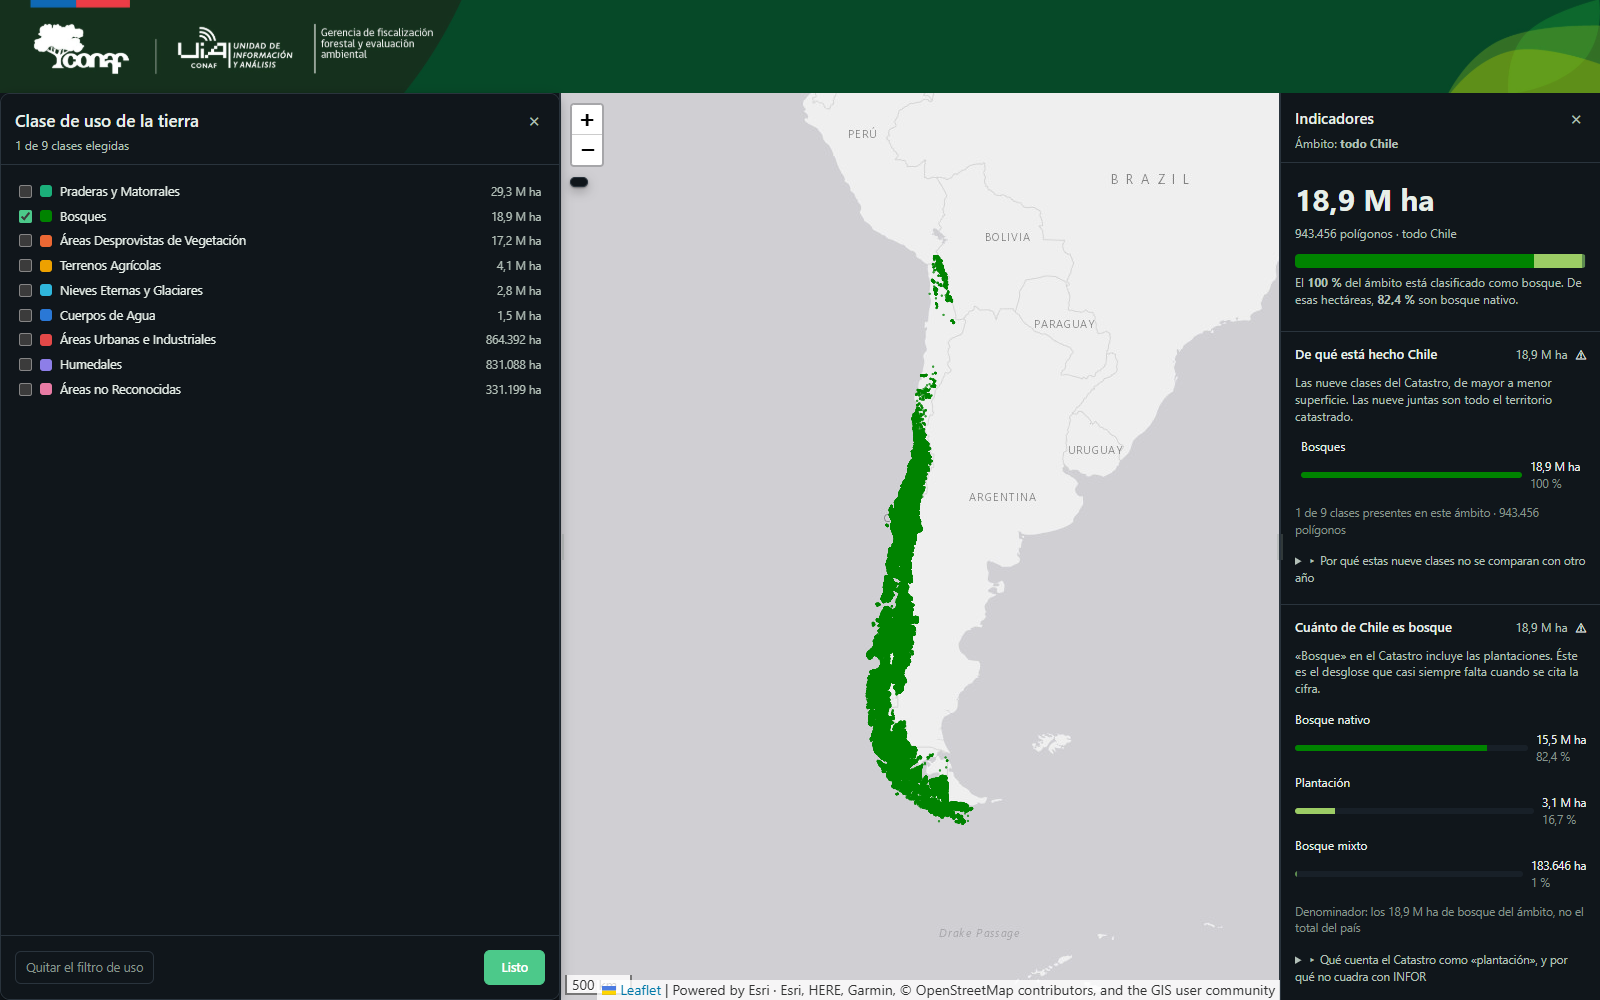
\includegraphics[width=\textwidth]{img/filtro-bosques.png}
\caption{Efecto de marcar sólo \emph{Bosques}: el mapa deja únicamente los
943.456 polígonos de bosque y el panel pasa de 75,7 a 18,9 millones de hectáreas.}
\end{figure}

\section{Un conjunto vacío no es «todas»}

\begin{alerta}
Si se desmarcan \emph{todas} las casillas de un filtro, eso significa
\campo{ninguna}, y el resultado queda vacío: no significa «todas». Para volver a
verlo todo hay que usar \campo{Quitar el filtro}, no desmarcar una por una.
\end{alerta}

% ----------------------------------------------------------------
\chapter{Cómo se lee el mapa}

\section{Qué es cada punto}

Cada punto es el \campo{centroide} del polígono que dibujó el Catastro. No es
una parcela, ni un predio, ni un árbol.

\begin{alerta}
El centroide de un polígono muy irregular puede caer \emph{fuera} de él. En un
polígono con forma de herradura, el punto marcado está en el hueco.
\end{alerta}

\section{El tamaño del punto}

El disco de cada punto ocupa la superficie que declara el polígono —el círculo
de igual área—, salvo donde no cabe: ahí se recorta hasta tocar a su vecino sin
invadirlo. Está recortado el \textbf{56\,\%} de los puntos (1.019.786 de
1.827.933), así que \campo{en zonas densas el tamaño ya no se puede leer como
superficie}. La cifra exacta está siempre en la ficha del punto, en los filtros
y en las descargas.

El radio mediano es de 67~m y el mayor llega a 13.130~m. A partir del zoom 11
ningún disco tapa a otro; alejando el mapa vuelven a tocarse, y eso no tiene
arreglo: son 1,8 millones de polígonos sobre unos 700.000 píxeles de pantalla.

\begin{nota}
\campo{Lo que el disco nunca reproduce es la forma.} Una faja estrecha de diez
kilómetros y un cuadrado compacto de la misma superficie se dibujan igual.
\end{nota}

\section{Los colores}

El color del punto indica su \campo{clase de uso}, con nueve colores fijos, para
que un enlace guardado siga significando lo mismo. Sólo el violeta de Humedales
se aclara en tema oscuro (\orig{\#4a3aa7} en claro, \orig{\#8d7ee8} en oscuro)
para que siga siendo legible; los otros ocho no cambian nunca.

\begin{center}
\begin{tabular}{@{}cl r@{}}
\toprule
& \textbf{Clase de uso} & \textbf{Superficie}\\
\midrule
\textcolor[HTML]{1baf7a}{\rule{3.2mm}{3.2mm}} & Praderas y Matorrales & 29.282.364,32 ha\\
\textcolor[HTML]{008300}{\rule{3.2mm}{3.2mm}} & Bosques & 18.862.754,85 ha\\
\textcolor[HTML]{eb6834}{\rule{3.2mm}{3.2mm}} & Áreas Desprovistas de Vegetación & 17.191.344,39 ha\\
\textcolor[HTML]{eda100}{\rule{3.2mm}{3.2mm}} & Terrenos Agrícolas & 4.088.178,65 ha\\
\textcolor[HTML]{2fb6dc}{\rule{3.2mm}{3.2mm}} & Nieves Eternas y Glaciares & 2.756.878,68 ha\\
\textcolor[HTML]{2a78d6}{\rule{3.2mm}{3.2mm}} & Cuerpos de Agua & 1.453.000,56 ha\\
\textcolor[HTML]{e34948}{\rule{3.2mm}{3.2mm}} & Áreas Urbanas e Industriales & 864.391,83 ha\\
\textcolor[HTML]{4a3aa7}{\rule{3.2mm}{3.2mm}} & Humedales & 831.088,25 ha\\
\textcolor[HTML]{e87ba4}{\rule{3.2mm}{3.2mm}} & Áreas no Reconocidas & 331.198,86 ha\\
\bottomrule
\end{tabular}
\end{center}

Los nueve colores se nombran, con su superficie al lado, dentro del filtro
\campo{Uso}. La paleta se eligió con un validador de contraste y de visión con
deficiencia de color, no a ojo; aun así, con nueve clases simultáneas el color
por sí solo no basta, y por eso la clase se nombra también en la ficha del punto
y en la tabla del panel.

\section{La ficha de un polígono}

Al pulsar un punto se abre su ficha con doce atributos.

\begin{figure}[htbp]
\centering
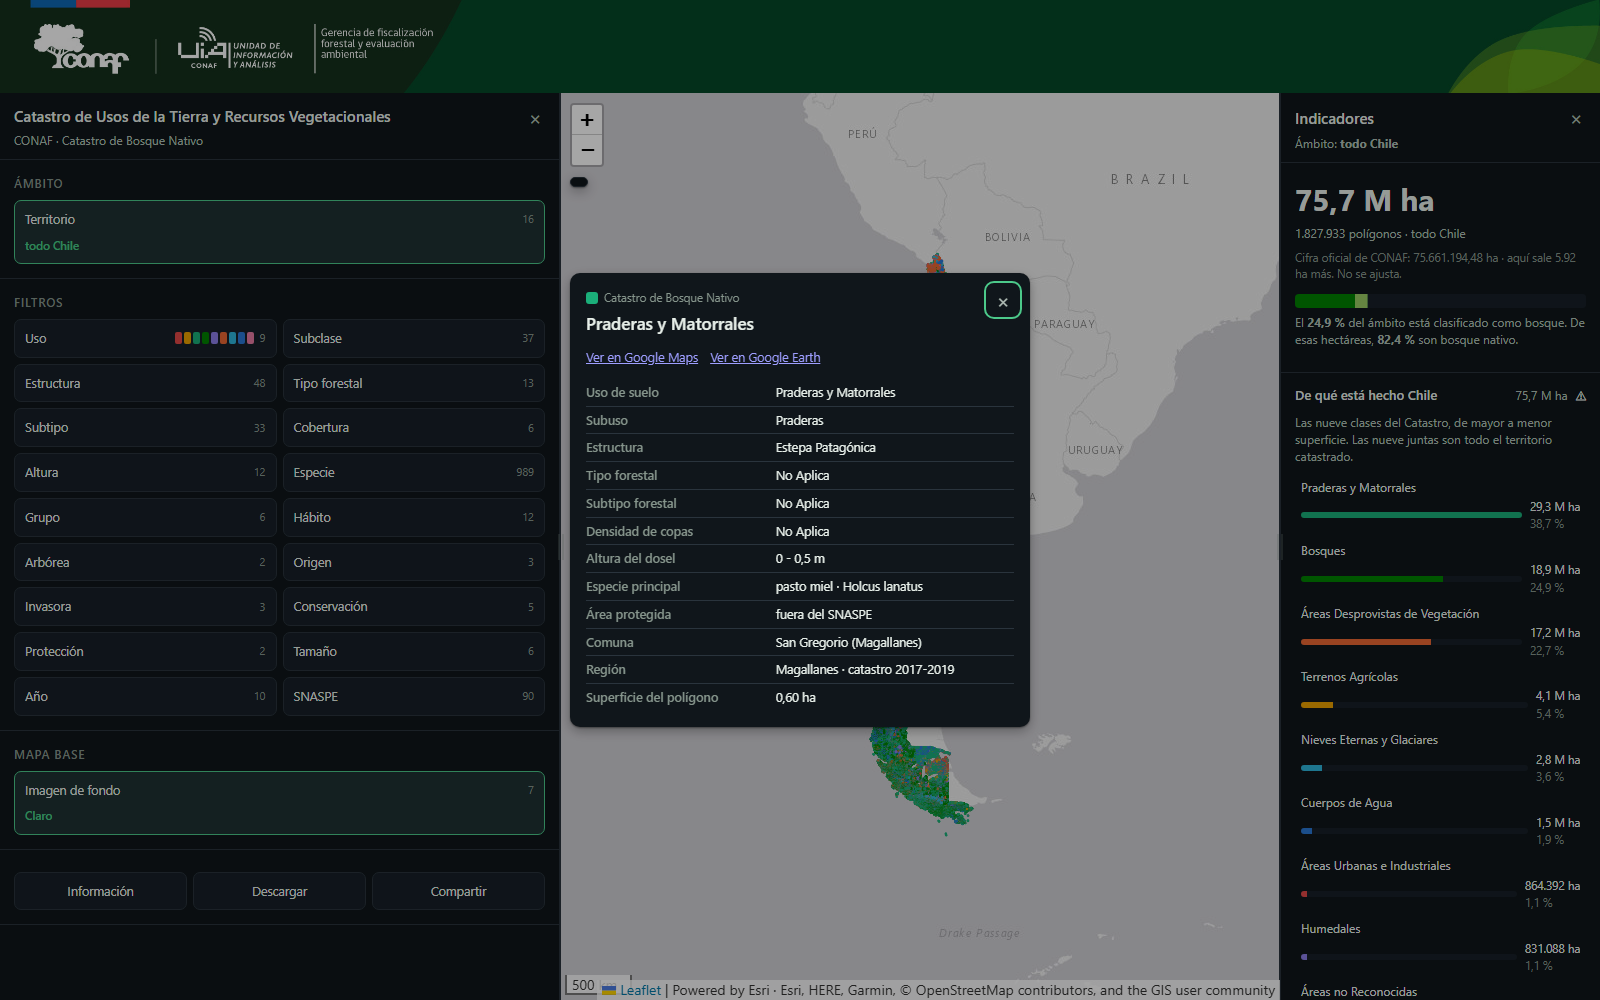
\includegraphics[width=\textwidth]{img/ficha-punto.png}
\caption{Ficha de un polígono. Incluye enlaces para abrir esa coordenada en
Google Maps y en Google Earth.}
\end{figure}

Los campos son: uso de suelo, subuso, estructura, tipo forestal, subtipo
forestal, densidad de copas, altura del dosel, especie principal (nombre común y
científico), área protegida, comuna, región con su año de catastro y superficie
del polígono.

\section{El mapa de fondo}

El control \campo{Imagen de fondo} ofrece siete opciones: \campo{Claro} (por
defecto), \campo{Oscuro}, \campo{Relieve}, \campo{Calles}, \campo{Topográfico},
\campo{Satelital} y \campo{Sentinel-2}. El propio modal lo advierte: «El fondo
no cambia ninguna cifra: sólo la imagen sobre la que se dibujan los polígonos.»

\begin{figure}[htbp]
\centering
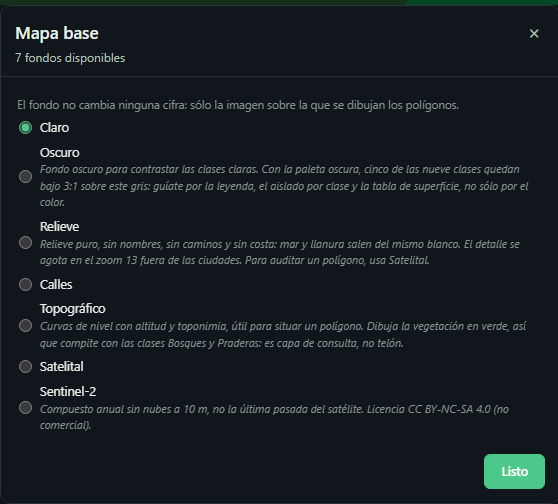
\includegraphics[width=0.52\textwidth]{img/modal-mapa-base.png}
\caption{Selector de mapa de fondo. Las opciones que tienen alguna advertencia
de lectura la explican debajo del nombre.}
\end{figure}

\begin{alerta}
La capa \campo{Sentinel-2} es un compuesto anual sin nubes de EOX con licencia
CC~BY-NC-SA 4.0, es decir, \campo{no comercial}. Los demás fondos tienen sus
propias condiciones, declaradas en la atribución del pie del mapa.
\end{alerta}

% ----------------------------------------------------------------
\chapter{El panel de indicadores}
\label{cap:indicadores}

Todo lo que muestra este panel está calculado sobre \campo{la selección
activa}, no sobre el país, salvo donde diga lo contrario. Arriba del todo se lee
siempre el ámbito vigente.

\begin{figure}[htbp]
\centering
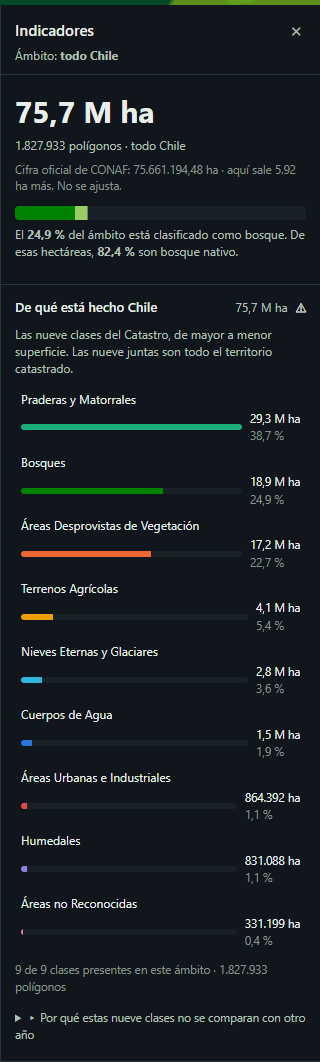
\includegraphics[height=0.62\textheight]{img/indicadores-1.png}
\hfill
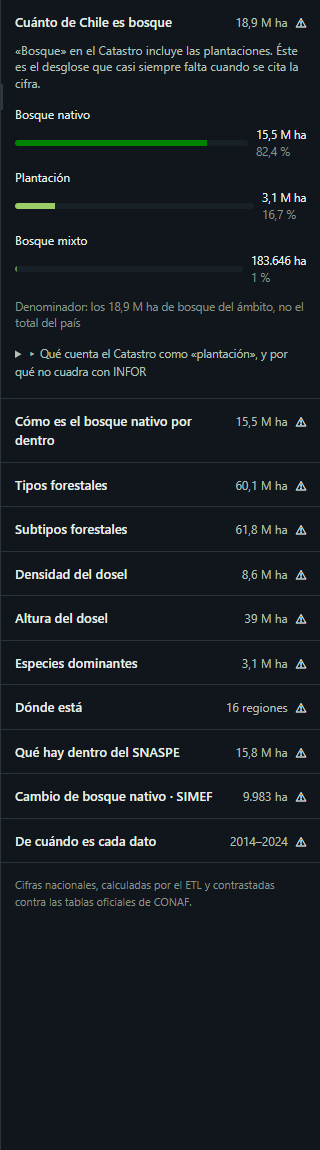
\includegraphics[height=0.62\textheight]{img/indicadores-2.png}
\caption{El panel de indicadores, en sus dos primeros tramos.}
\end{figure}

\section{La cifra de cabecera}

La superficie total de la selección, en millones de hectáreas, con el número de
polígonos debajo. Sin filtros: \textbf{75,7 M ha} y \textbf{1.827.933
polígonos}.

Debajo, el propio visor declara su diferencia con la cifra oficial:

\begin{nota}
El panel declara la cifra oficial de CONAF —75.661.194,48~ha—, dice cuánto se
aparta la suya (5,92~ha más) y advierte de que \campo{no se ajusta}.

Son 5,92 hectáreas sobre 75,6 millones: un 0,0000078\,\%. No se corrige a mano
porque no hay una causa verificada, y se prefiere declararlo a inventar una.
\end{nota}

\section{Las secciones}

Son doce, en este orden:

\begin{enumerate}
  \item \campo{De qué está hecho Chile} — las nueve clases de uso, de mayor a
        menor, con barra, hectáreas y porcentaje, más una tabla con el conteo de
        polígonos.
  \item \campo{Cuánto de Chile es bosque} — el desglose que casi siempre falta:
        de los 18,9 M ha de bosque, \textbf{82,4\,\%} es bosque nativo,
        \textbf{16,7\,\%} plantación y \textbf{1\,\%} bosque mixto.
  \item \campo{Cómo es el bosque nativo por dentro} — por estructura.
  \item \campo{Tipos forestales}.
  \item \campo{Subtipos forestales}.
  \item \campo{Densidad del dosel}.
  \item \campo{Altura del dosel}.
  \item \campo{Especies dominantes}.
  \item \campo{Dónde está} — reparto por región.
  \item \campo{Qué hay dentro del SNASPE}.
  \item \campo{Cambio de bosque nativo · SIMEF} — de otra fuente, no una
        continuación del Catastro. Cada par de años cubre un conjunto distinto
        de regiones, así que sus barras no se comparan entre sí. Muestra
        \campo{sólo las pérdidas} —deforestación y sustitución—: las clases de
        ganancia que SIMEF también registra, «Aumento» y «Restitución», no están
        en el visor. Esta sección \campo{no es un balance neto} y no debe
        leerse como tal.
  \item \campo{De cuándo es cada dato} — el año de levantamiento de cada región.
\end{enumerate}

Cada sección lleva un triángulo \textbf{\textcolor{aviso}{$\triangle$}} que
despliega la advertencia de lectura que le corresponde. Conviene abrirlos: ahí
está, por ejemplo, por qué las nueve clases no se comparan con otro año, o por
qué la cifra de plantaciones no cuadra con la de INFOR.

\section{Tres lecturas que se hacen mal}

\subsection{Contar polígonos no es medir superficie}
Un polígono de 0,1~ha y otro de 1.295.122~ha cuentan igual en el conteo y no en
las hectáreas. Para superficie, siempre las hectáreas.

\subsection{La especie es sólo la dominante}
Cada polígono puede registrar hasta seis especies. El visor filtra y suma por la
\campo{primera}, la dominante, y le asigna la superficie entera del polígono. No
es una convención propia: es la misma de la planilla oficial de plantaciones por
especie, y reproducirla da 1.714.737,31~ha de \emph{Pinus radiata} frente a las
1.714.736,78~ha publicadas por CONAF.

\subsection{La altura viene en dos escalas que se solapan}
Una da tramos en metros y la otra sólo distingue por encima y por debajo de
2~m. «Menos de 2~m» cubre lo mismo que los tres primeros tramos finos juntos,
así que sumar las dos escalas cuenta dos veces el mismo rango. El visor las
mantiene separadas en el panel, en el filtro y en el CSV.

\section{El filtro de estado de conservación}
\label{sec:conservacion}

\begin{alerta}
\campo{El Catastro no registra el estado de conservación de las especies.} No
hay ninguna columna de categoría de amenaza en ninguna de sus capas.

El filtro \campo{Conservación} de este visor no viene del Catastro: sale de una
tabla auxiliar de la Unidad de Información y Análisis que clasifica las 989
especies del vocabulario. Esa tabla \campo{no está validada} contra el
Reglamento de Clasificación de Especies (RCE) y sólo trae categoría para
\textbf{trece} especies: las otras \textbf{976} figuran como «Sin dato --- no
verificado en RCE».

Eso significa \emph{que no se ha comprobado}, no que la especie esté fuera de
peligro. Leer ese filtro como un inventario de especies amenazadas lo lee
exactamente al revés. Y que una especie aparezca con poca superficie tampoco
significa que esté amenazada: para eso está el inventario oficial del RCE, que
es otra fuente.
\end{alerta}

% ----------------------------------------------------------------
\chapter{Qué se puede llevar, y cómo}

El botón \campo{Descargar} abre las cuatro salidas. Todas respetan el ámbito y
los filtros activos.

\begin{figure}[htbp]
\centering
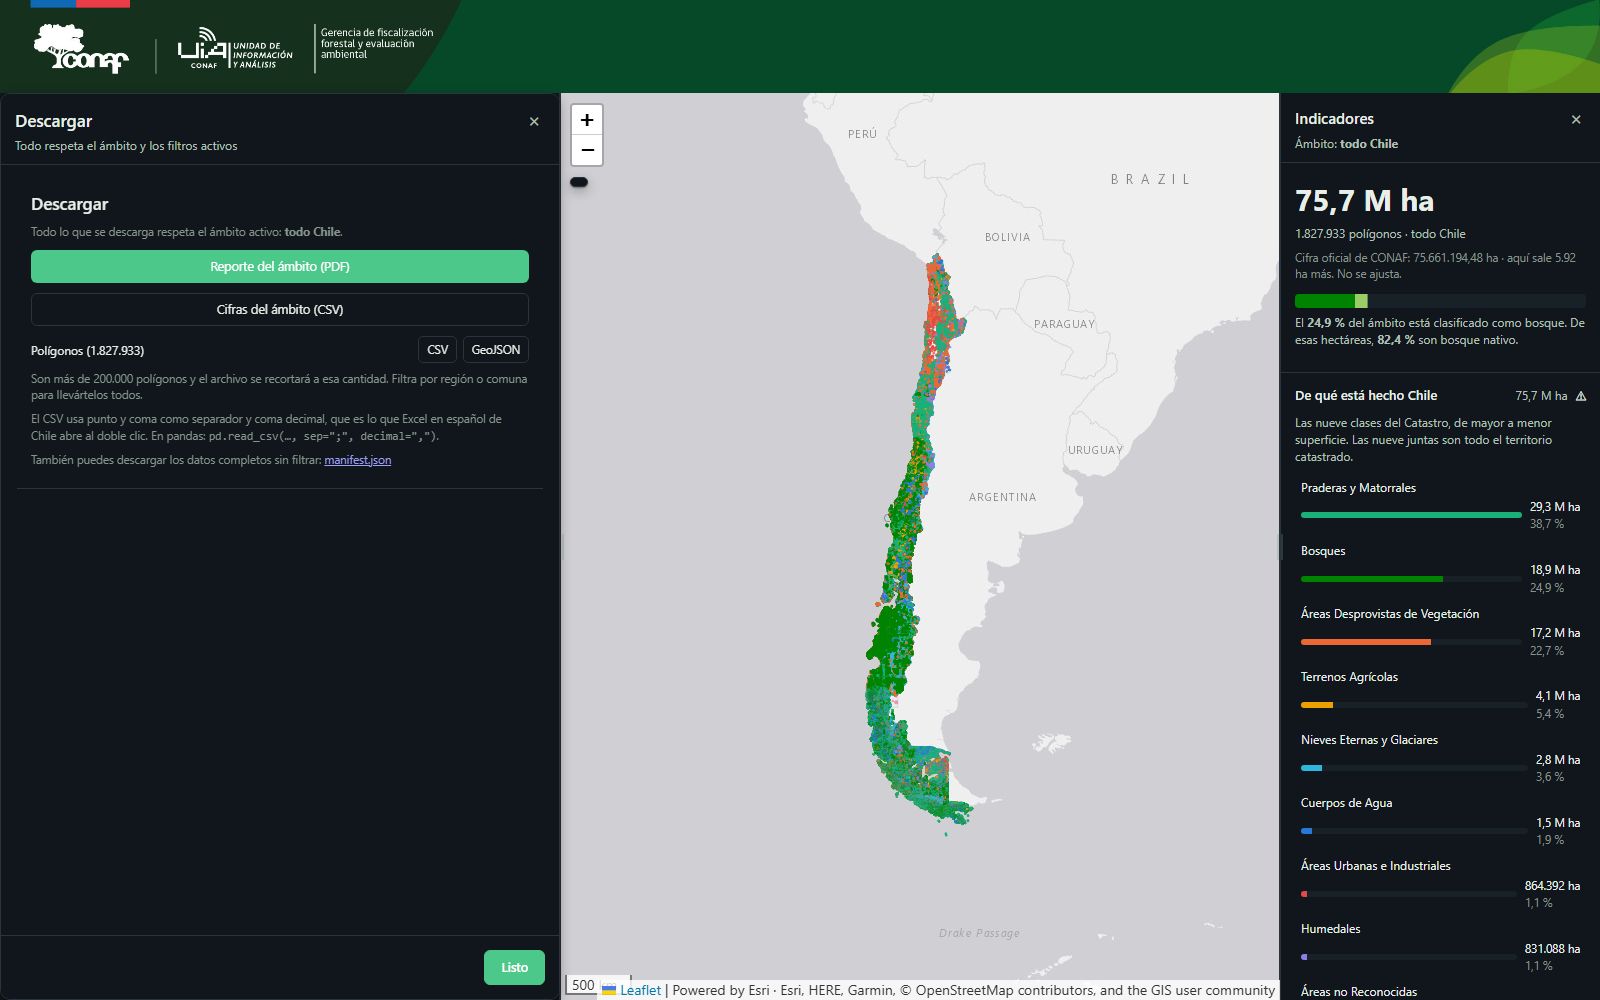
\includegraphics[width=\textwidth]{img/modal-descargar.png}
\caption{El modal de descargas, con el ámbito activo declarado arriba.}
\end{figure}

\section{Reporte del ámbito (PDF)}

Es la salida más completa: un documento institucional, listo para imprimir o
adjuntar, que se arma en el momento con el ámbito y los filtros que estén
puestos. Al pulsarlo, el visor \campo{congela la imagen del mapa tal como está
en pantalla} —con su encuadre, sus filtros y su fondo— y la incrusta en la
portada del reporte.

\begin{nota}
\campo{Para guardarlo:} el reporte se abre en pantalla con una barra superior
que trae \campo{Exportar PDF}. Ese botón abre el diálogo de impresión del
navegador, donde hay que elegir «Guardar como PDF» como destino. El botón
\campo{← Cerrar} vuelve al visor.
\end{nota}

\begin{figure}[htbp]
\centering
\fbox{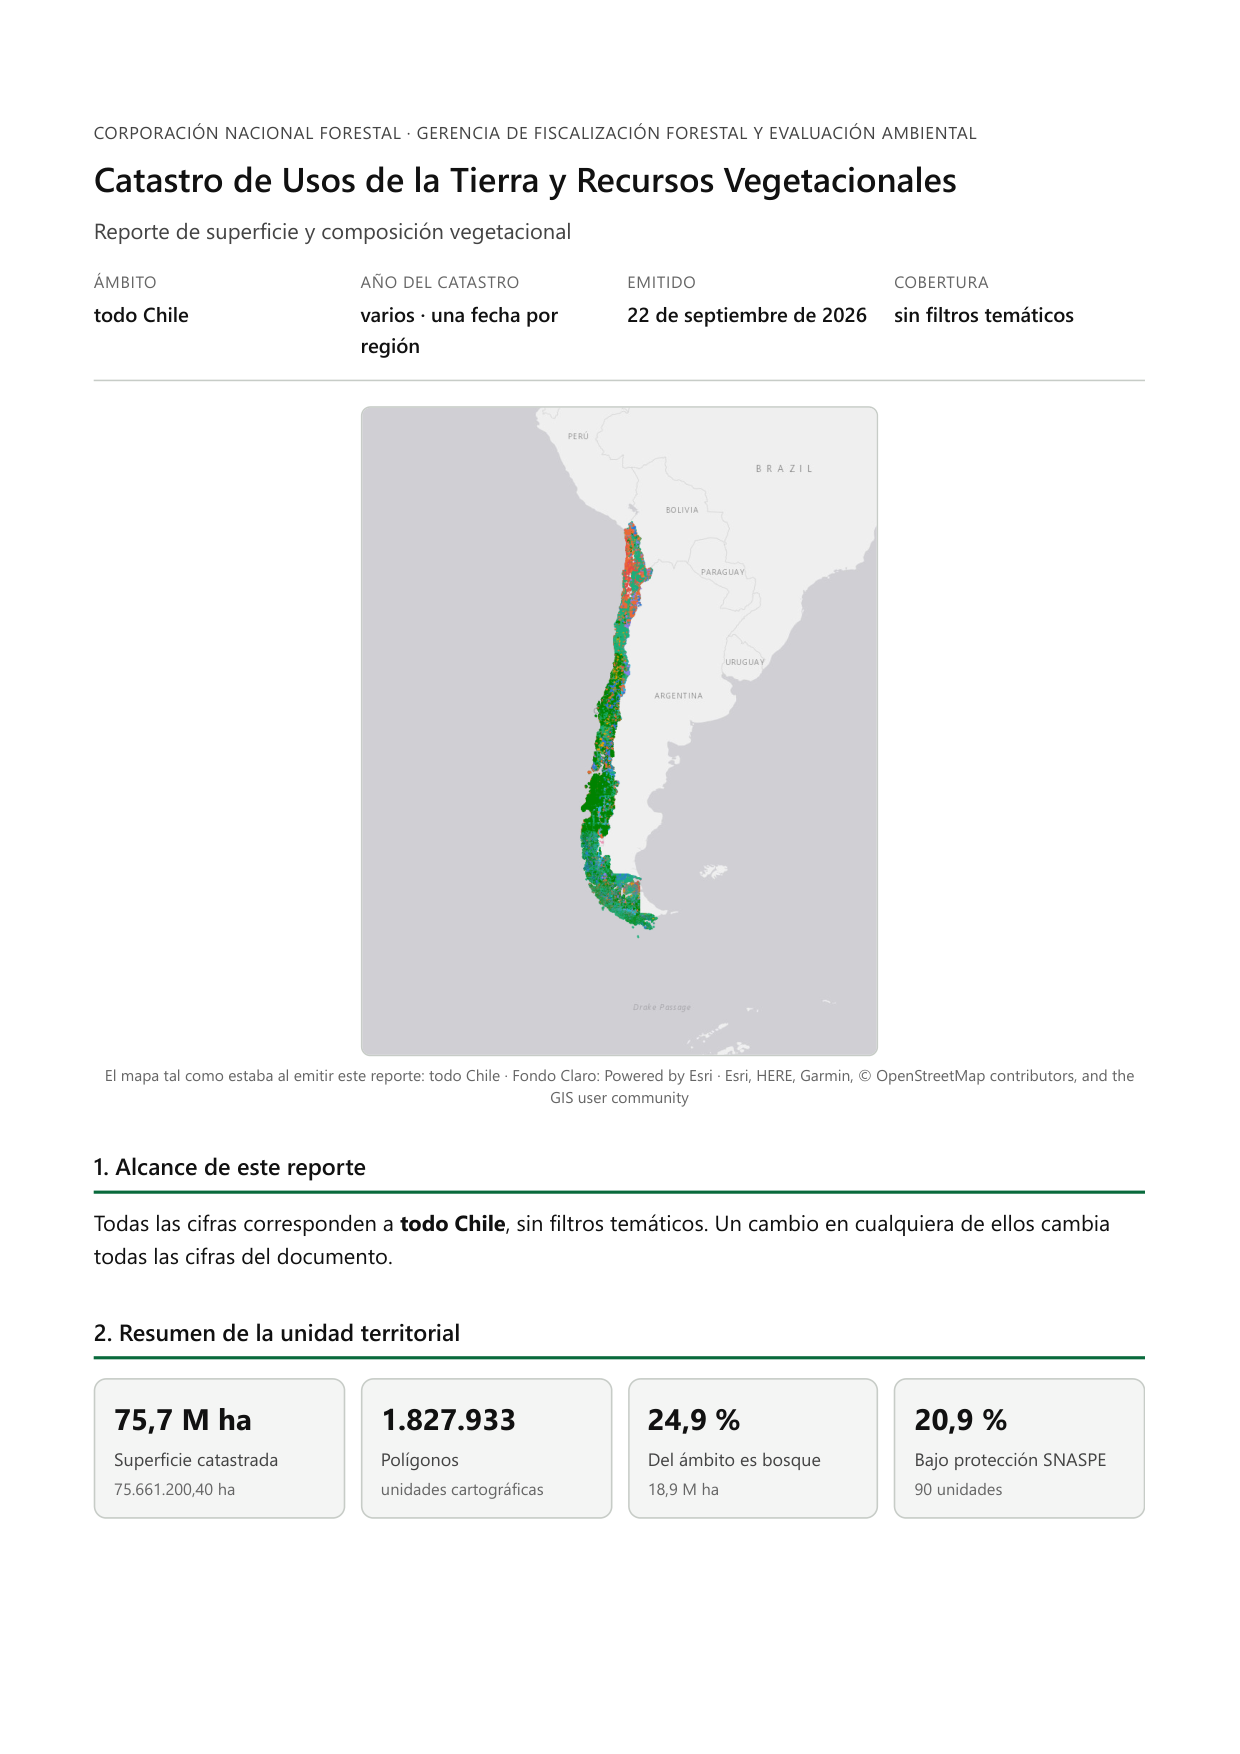
\includegraphics[width=0.45\textwidth]{img/reporte-p1.png}}
\hfill
\fbox{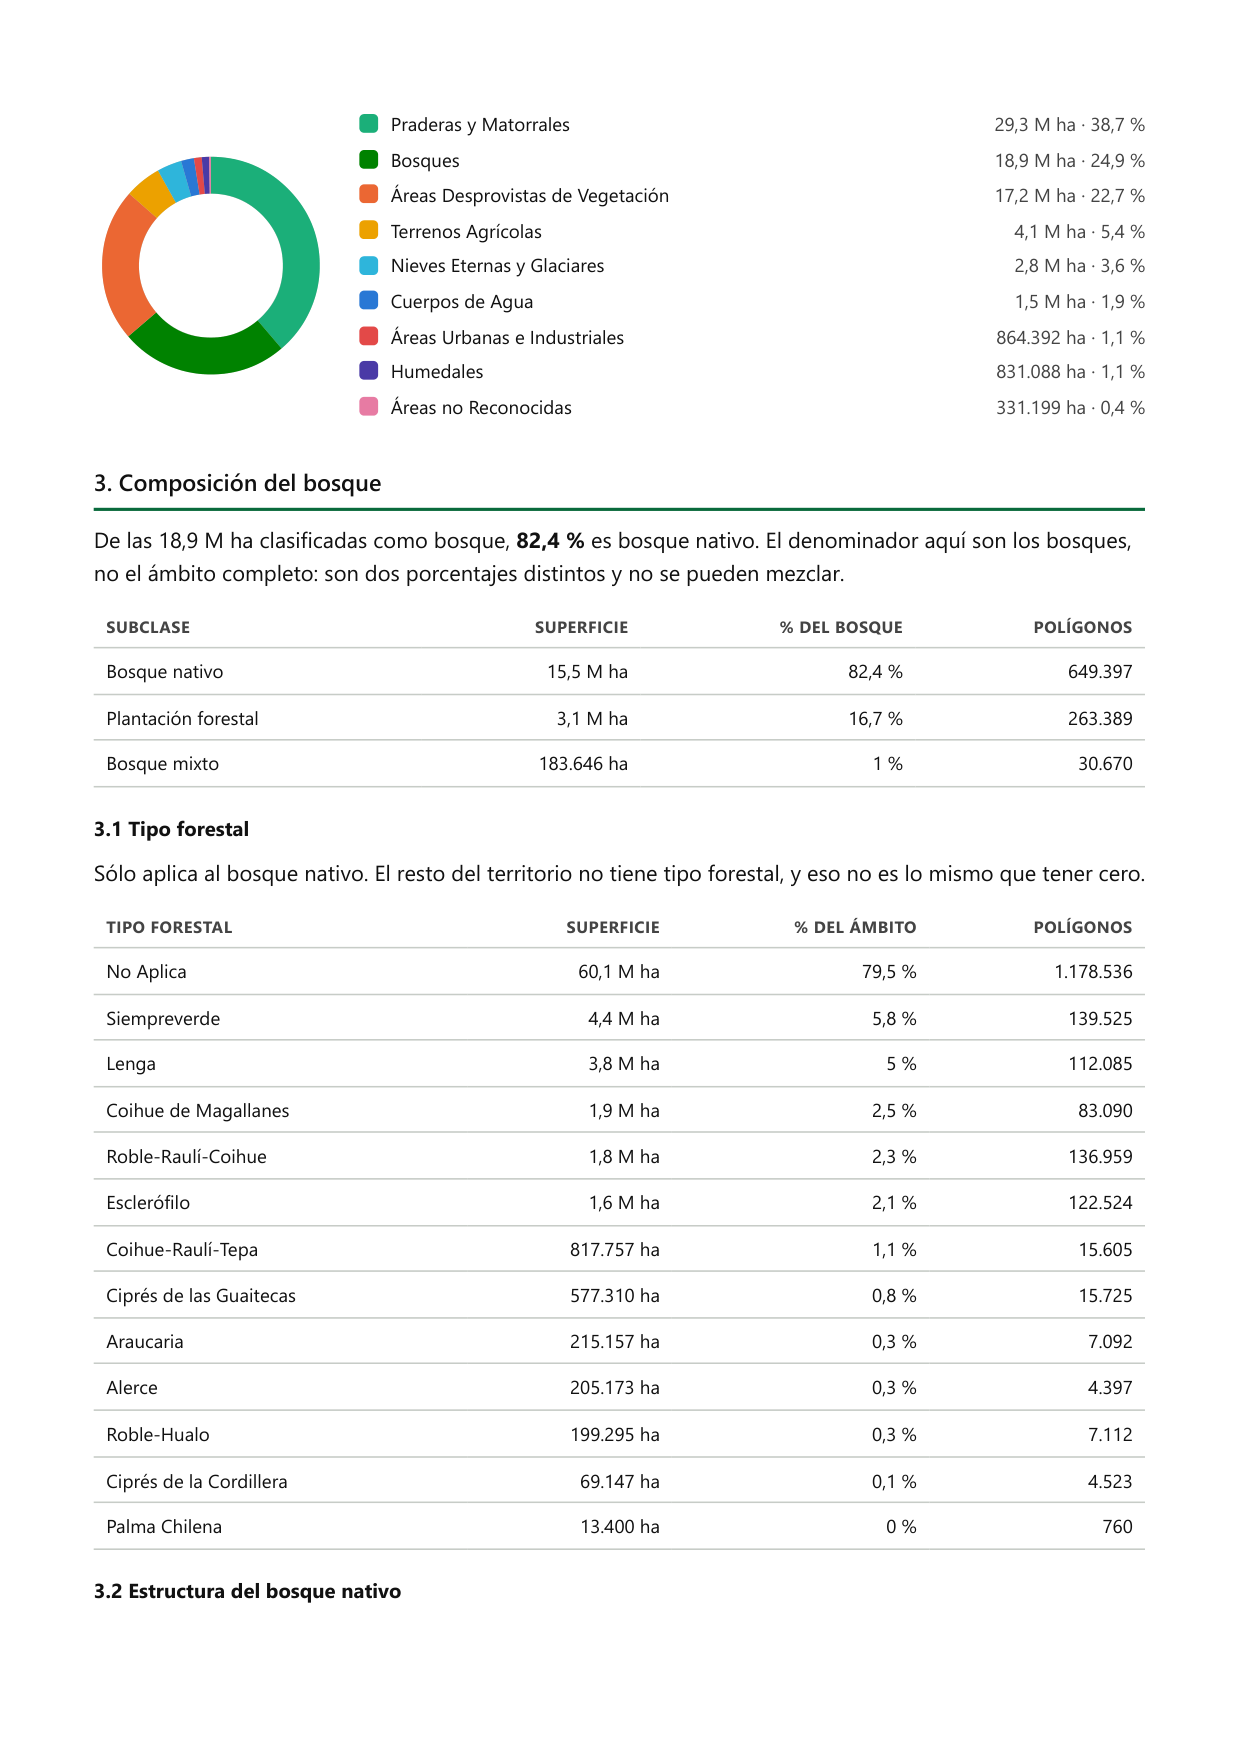
\includegraphics[width=0.45\textwidth]{img/reporte-p2.png}}
\caption{Las dos primeras páginas del reporte generado sin filtros, tal como
salen de «Exportar PDF». El documento completo tiene ocho páginas y se adjunta
a este manual como \texttt{ejemplo-reporte-del-visor.pdf}.}
\end{figure}

El reporte trae ocho secciones y tres anexos:

\begin{enumerate}[itemsep=1pt]
  \item \campo{Alcance de este reporte} — qué ámbito y qué filtros se aplicaron.
  \item \campo{Resumen de la unidad territorial} — superficie, número de
        polígonos, porcentaje de bosque, porcentaje bajo protección, y el
        reparto por las nueve clases de uso.
  \item \campo{Composición del bosque} — nativo, plantación y mixto.
  \item \campo{Estado de protección} — dentro y fuera del SNASPE.
  \item \campo{Estructura del dosel}.
  \item \campo{Especies principales}.
  \item \campo{Distribución territorial} — por región o comuna, cada una con su
        año de catastro.
  \item \campo{Cobertura del dato} — cuántos polígonos no traen cada atributo.
  \item[] \campo{Anexo A} — las clases de uso, con superficie y porcentaje.
  \item[] \campo{Anexo B} — las subclases de uso, con su clase madre.
  \item[] \campo{Anexo C} — «Qué no dice este reporte»: las advertencias de
        lectura, en la última página. Es la que conviene no arrancar al
        reenviarlo.
\end{enumerate}

\begin{nota}
\campo{La sección 8 es la que conviene leer siempre.} Dice cuántos polígonos
del ámbito no traen cada dato, y esos no se reparten entre las clases ni cuentan
como cero: quedan fuera de los porcentajes. Sin filtros, por ejemplo, el
42,7\,\% de los polígonos no tiene altura del dosel y el 15,6\,\% no tiene
especie principal.
\end{nota}

\section{Cifras del ámbito (CSV)}
Las tablas del panel de indicadores, en formato de planilla.

\section{Los polígonos (CSV o GeoJSON)}

\begin{alerta}
\campo{Hay un tope de 200.000 polígonos por archivo.} Sin filtros son 1.827.933
y la descarga se recorta. Para llevarse todos los de un territorio hay que
filtrar antes por región o comuna.
\end{alerta}

\begin{nota}
\campo{El CSV está hecho para Excel en español de Chile:} separador punto y
coma, coma decimal. Se abre con doble clic sin pasar por el asistente de
importación. En \texttt{pandas}:

\begin{center}
\orig{pd.read\_csv(..., sep=";", decimal=",")}
\end{center}
\end{nota}

\section{manifest.json}
El catálogo completo de todos los vocabularios, con sus códigos, etiquetas,
conteos y superficies, sin filtrar. Es el archivo que conviene pedir cuando
alguien quiere replicar estas cifras.

\section{Compartir una vista}

El botón \campo{Compartir} da un enlace que guarda \campo{el ámbito, todos los
filtros, el mapa base y el encuadre}. Quien lo abra verá exactamente las mismas
cifras.

\begin{alerta}
Ese enlace muestra cifras \emph{de la selección}, no las nacionales. Al pegarlo
en un correo conviene decir qué selección es.
\end{alerta}

% ----------------------------------------------------------------
\chapter{Tres consultas, paso a paso}

\section{Cuánto bosque nativo hay en una región}
\begin{enumerate}
  \item \campo{Territorio} → marcar la región → \campo{Listo}.
  \item \campo{Uso} → marcar \emph{Bosques} → \campo{Listo}.
  \item \campo{Subclase} → marcar \emph{Bosque Nativo} → \campo{Listo}.
  \item La cifra de cabecera del panel derecho es la respuesta. El desglose por
        estructura y por tipo forestal está más abajo, en el mismo panel.
  \item \campo{Descargar} → \emph{Reporte del ámbito (PDF)} para dejarlo por escrito.
\end{enumerate}

\section{Dónde hay araucaria dentro de áreas protegidas}
\begin{enumerate}
  \item \campo{Tipo forestal} → marcar \emph{Araucaria}.
  \item \campo{Protección} → marcar \emph{Dentro del SNASPE}.
  \item El mapa deja sólo esos polígonos; \campo{SNASPE} permite además bajar a
        una unidad concreta.
  \item Pulsar cualquier punto abre su ficha con la comuna, la superficie y el
        año del levantamiento.
\end{enumerate}

\section{Los polígonos grandes de plantación de una comuna}
\begin{enumerate}
  \item \campo{Territorio} → elegir la comuna.
  \item \campo{Subclase} → \emph{Plantación}.
  \item \campo{Tamaño} → \emph{100--500 ha} y \emph{500 ha o más}.
  \item \campo{Descargar} → \emph{Polígonos · GeoJSON}, que abre directamente en
        QGIS o ArcGIS.
\end{enumerate}

% ================================================================
\part{Qué se le cambió a los datos respecto de la base original}
% ================================================================

\chapter{Para qué sirve esta segunda parte}

El visor no publica el Catastro tal como sale de la base: lo normaliza. Esta
parte registra \campo{todos} esos cambios, con la cifra medida al lado, para que
cualquiera pueda contrastar una cifra del visor con la fuente y saber por qué
difiere —o por qué no debería diferir.

\begin{nota}
\campo{Qué se entiende aquí por «base original».} Lo que el proceso lee no es el
archivo de terreno de la Unidad, sino una base intermedia
(\orig{data/catastro\_gef\_singeometria.duckdb}, 300.691.456 bytes) que consolida
\textbf{22 coberturas regionales} —16.427,8~MB de origen— a las que ya se les
quitó la geometría, se les precalculó el centroide y se les aplicaron
\textbf{349 reparaciones de texto} registradas en la propia base. Todo lo que
sigue compara \emph{esa} base contra lo publicado. Parte del ruido de
codificación de caracteres ya venía reparado de antes, así que este registro no
puede atribuirse la totalidad de la limpieza.
\end{nota}

\section{El resumen, en una tabla}

\begin{longtable}{@{}L{6.6cm} r r@{}}
\toprule
\textbf{} & \textbf{En la base} & \textbf{Publicado}\\
\midrule
\endfirsthead
\toprule
\textbf{} & \textbf{En la base} & \textbf{Publicado}\\
\midrule
\endhead
Polígonos & 1.827.934 & 1.827.933\\
Superficie total (ha) & 75.661.200,40 & 75.661.200,40\\
Columnas de atributos & 91 & 27 leídas\\
Grafías de clase de uso & 14 & 9 clases\\
Grafías de subclase & 62 & 43 entradas\\
Grafías de estructura & 31 & 19 etiquetas\\
Grafías de tipo forestal & 19 & 13 clases\\
Grafías de subtipo forestal & 39 & 33 clases\\
Grafías de cobertura & 12 & 6 clases\\
Grafías de altura & 24 & 12 clases\\
Rótulos de unidad del SNASPE & 94 & 90 unidades\\
Códigos de especie & 991 & 989 especies\\
\bottomrule
\caption{El antes y el después, medido sobre la base y sobre el archivo publicado.}
\end{longtable}

\begin{nota}
\campo{La superficie total no cambia.} Ninguna de las transformaciones que
siguen suma ni resta hectáreas: reagrupan, renombran y completan, pero el total
del origen y el del sitio coinciden al céntimo.
\end{nota}

% ----------------------------------------------------------------
\chapter{Qué filas y qué columnas entran}

\section{Se descarta exactamente un polígono}

Entran 1.827.934 filas y salen 1.827.933. La única que se cae es un polígono
vacío de la Región del Maule: sin atributos, 0 hectáreas y \campo{sin centroide}
—el campo viene vacío, y sus coordenadas UTM son (0,\,0)—. No hay ninguna otra
exclusión, ni deduplicación, ni agregación: \campo{cada polígono del Catastro es
un punto del mapa}.

\section{De 91 columnas se leen 27}

Las 64 restantes se descartan, y conviene decir cuáles, porque alguien las va a
echar de menos:

\begin{itemize}
  \item \campo{Las cinco especies secundarias} de cada polígono: 1.165.029 filas
        traen al menos una. Sólo viaja la especie dominante, y ésa es la razón
        de que el visor no pueda decir qué acompaña a la especie principal.
  \item \campo{Las coordenadas UTM} (\orig{COOR\_ESTE}, \orig{COOR\_NORTE}):
        valen exactamente 0 en 1.546.956 filas y sólo 99.048 traen un valor
        utilizable. La ubicación publicada sale del centroide precalculado, no
        de ellas.
  \item \campo{El bloque de reclasificación de bosque nativo} (diez columnas):
        sólo está poblado en parte del país, así que publicarlo daría una
        segunda clasificación paralela e incompleta.
  \item \campo{Los códigos de terreno del catastrador} (\orig{FV\_CONAF},
        \orig{ED\_CONAF}): 1.610 y 2.025 valores distintos, ilegibles fuera de la
        Unidad («\orig{Er/mr1/b23 a46 al1}»).
  \item \campo{Las columnas de texto que duplican un código}, por el motivo del
        capítulo siguiente.
  \item Identificadores internos, columnas vacías y columnas constantes.
\end{itemize}

\section{Once atributos cambian de nombre, y tres se recomponen}

Los nombres técnicos se acortan al publicarse. Tres de los cambios no son un
renombre sino una \campo{recomposición}, y explicarlo evita un error de lectura:

\begin{longtable}{@{}L{6.2cm} L{6.2cm}@{}}
\toprule
\textbf{En la base} & \textbf{Publicado}\\
\midrule
\endhead
\orig{centroide\_lon} / \orig{centroide\_lat} & \orig{lon} / \orig{lat}\\
\orig{SUPERF\_HA} & \orig{ha}\\
\orig{COALESCE(CODCOM, Codcomun)} & \orig{comuna}\\
\orig{ID\_USO} & \orig{uso}\\
\orig{ID\_USO + ID\_SUBUSO} & \orig{subuso} (código de 4 dígitos)\\
\orig{ID\_USO + ID\_SUBUSO + ID\_ESTRUC} & \orig{estruc} (código de 6 dígitos)\\
\orig{ID\_ESP1} & \orig{especie}\\
\orig{ID\_TIFO} & \orig{tifo} (tipo forestal)\\
\orig{SUBTIPOFOR} & \orig{stifo} (subtipo forestal)\\
\orig{ID\_COBER} & \orig{cober} (cobertura)\\
\orig{ID\_ALTU} & \orig{altura}\\
\orig{NOM\_SNASPE} & \orig{snaspe}\\
\orig{reg\_cod} & \orig{region}\\
\bottomrule
\end{longtable}

\begin{alerta}
\campo{Por qué se concatenan los códigos.} Los códigos de subclase y estructura
son \emph{relativos a su padre}: el «01» de estructura significa una cosa dentro
de Praderas y otra dentro de Bosques. Sólo el código largo es único. Quien
cruce estos datos por el código corto obtendrá mezclas sin ningún aviso.
\end{alerta}

\begin{nota}
\campo{La comuna se lee de dos columnas distintas.} La Región de Los Ríos guarda
el código comunal en \orig{Codcomun} y no en \orig{CODCOM}. Sin ese doble
intento, sus 79.727 polígonos y 1.835.307,15~ha se quedaban sin desglose
comunal.
\end{nota}

% ----------------------------------------------------------------
\chapter{La limpieza del texto}

\section{Qué hace exactamente}

Toda comparación de texto pasa por una función de canonización que hace cuatro
cosas, y sólo cuatro:

\begin{enumerate}[itemsep=1pt]
  \item cambia el guion tipográfico (\,–\,, \,—\,) por el guion normal;
  \item cambia el espacio duro por espacio normal;
  \item colapsa espacios repetidos y saltos de línea en uno solo, y recorta los
        de los extremos;
  \item ignora mayúsculas y signos diacríticos \emph{al comparar} —incluidas la
        tilde de la ñ y la diéresis: «Ñuble» y «Nuble» son la misma clave.
\end{enumerate}

\begin{nota}
\campo{Se usa para agrupar, no para mostrar.} La etiqueta que acaba en pantalla
es la grafía \emph{más frecuente} del grupo, tal como la escribe el Catastro,
con sus mayúsculas y sus tildes. La normalización no reescribe el Catastro: sólo
decide qué valores son el mismo.
\end{nota}

\section{Un caso concreto: la clase de altura «2 - 4»}

En la base, los polígonos de esa clase traen el texto escrito de cinco maneras:

\begin{center}
\begin{tabular}{@{}lrr@{}}
\toprule
\textbf{Texto en la base} & \textbf{Polígonos} & \textbf{Hectáreas}\\
\midrule
\orig{2 - 4} & 111.128 & 1.908.462,54\\
\orig{2 – 4} \small(guion largo) & 9.576 & 114.014,51\\
\orig{2 - 4\textbackslash n} \small(con salto de línea) & 3.050 & 42.379,25\\
\orig{2-4} \small(sin espacios) & 1.818 & 79.591,72\\
\orig{0-2} \small(otra clase, sólo en Arica) & 629 & 42.681,27\\
\midrule
\textbf{Clase A publicada} & \textbf{126.201} & \textbf{2.187.129,29}\\
\bottomrule
\end{tabular}
\end{center}

Quien filtrara por la grafía más frecuente en lugar de por la clase se dejaría
fuera \campo{278.666,75 hectáreas, el 12,7\,\% de la clase}.

\begin{alerta}
\campo{Quien agrupa aquí es el código, no la limpieza del texto.} Los cinco
textos comparten el código \orig{ID\_ALTU = 'A'}, y es ese código el que forma
la clase. La canonización no habría bastado: funde los tres primeros, pero deja
fuera \orig{2-4} —sin espacios— y sobre todo \orig{0-2}, que dice otra cosa.

Es el argumento de fondo de todo este capítulo: \campo{donde hay código
oficial, manda el código}; el texto sólo decide qué etiqueta se muestra. La
limpieza del texto agrupa únicamente donde no hay código utilizable.
\end{alerta}

En cobertura ocurre lo mismo: «Muy Abierto» convive con «Muy abierto» (12.704
polígonos) y «Muy Abierta» (438), y los tres son la misma clase porque comparten
código.

\section{Dónde NO se normaliza, a propósito}

\begin{alerta}
\campo{El código de especie distingue mayúsculas y minúsculas.} Medido sobre el
catálogo publicado: de los 989 códigos, hay \textbf{205 grupos} —466 códigos en
total— que sólo se diferencian en la caja de las letras, y designan especies
distintas. Un \orig{upper()} sobre esa columna dejaría 728 códigos:
\campo{fundiría 261 especies en silencio}, sin error y sin que las cifras
dejaran de cuadrar.

\begin{center}
\begin{tabular}{@{}llrr@{}}
\toprule
\textbf{Código} & \textbf{Especie} & \textbf{Polígonos} & \textbf{Hectáreas}\\
\midrule
\orig{AB} & \emph{Abies} sp. & 2 & 6,30\\
\orig{Ab} & \emph{Adesmia boronioides} & 141 & 21.510,03\\
\orig{ab} & \emph{Calceolaria biflora} & 18 & 43,46\\
\bottomrule
\end{tabular}
\end{center}
\end{alerta}

Por la misma razón, la unión se hace siempre \campo{por código y nunca por
nombre}: en el catálogo publicado, \textbf{48 nombres comunes} designan más de
una especie. El extremo es «quisco», que corresponde a doce códigos distintos;
le siguen «coirón» con ocho y «eucalipto» con siete.

\begin{nota}
\campo{Una excepción medida.} De los 205 grupos, en 204 todos los códigos son
especies distintas. En uno —\orig{DD}, \orig{Dd}, \orig{dD}, \orig{dd}— dos de
los cuatro (\orig{Dd} y \orig{dD}) son la misma especie, \emph{Desfontainia
fulgens}. Es uno de los casos que siguen esperando decisión.
\end{nota}

\section{Por qué la etiqueta sale del código y no del texto}

Donde existe un código oficial, la etiqueta y los agregados salen de él. La
razón está medida: agregando la estructura del bosque nativo \emph{por texto} se
quedaban fuera \textbf{95.626,20 hectáreas} en 1.516 polígonos, que resultaron
ser las regiones de Coquimbo y Arica y Parinacota enteras. No era una cuestión
de tildes: cada una usa un nombre propio que la limpieza del texto no puede
adivinar.

\begin{center}
\begin{tabular}{@{}L{3.7cm} L{4.1cm} L{2.9cm} r@{}}
\toprule
\textbf{Región} & \textbf{Escribe} & \textbf{El resto del país} & \textbf{Hectáreas}\\
\midrule
Coquimbo & \orig{Bosque Adulto} & \orig{Adulto} & 48.474,86\\
Arica y Parinacota & \orig{Bosque Adulto/Renoval} & \orig{Adulto-Renoval} & 47.151,34\\
\bottomrule
\end{tabular}
\end{center}

% ----------------------------------------------------------------
\chapter{La tabla de homologación}

\section{Qué es y de dónde sale}

Encima de la limpieza automática se aplica una tabla de equivalencias
\campo{revisada por la Unidad de Información y Análisis}, no una regla
automática. Su fuente es un libro Excel de la Unidad
(\orig{INSUMO/homologacion\_catastro\_1.xlsx}, fechado el 29 de agosto de 2026),
con 17 hojas, que se convierte a CSV versionados para que cualquier corrección
quede visible en el historial en vez de esconderse dentro de un binario.

\section{Cuántos cambios son, en total}

De \textbf{1.630 equivalencias}, sólo \textbf{89 cambian realmente el valor}:
81 se aplican y 8 quedan sin aplicar a propósito.

\begin{center}
\begin{tabular}{@{}lrL{7.4cm}@{}}
\toprule
\textbf{Acción} & \textbf{Filas} & \textbf{Qué significa}\\
\midrule
\orig{sin\_cambio} & 1.538 & El valor se publica tal cual.\\
\orig{ortografia} & 52 & Se repone una tilde, una ñ o una diéresis, o se corrige un tipeo.\\
\orig{fusion} & 13 & Dos grafías de lo mismo pasan a ser una clase.\\
\orig{prefijo} & 13 & Se antepone la categoría al nombre de la unidad.\\
\rowcolor{filagris} \orig{revisar} & 8 & \textbf{No se aplica}: exige decisión institucional.\\
\orig{codificacion} & 3 & Se repara un carácter corrompido.\\
\orig{formato} & 2 & Se ajusta el separador decimal.\\
\rowcolor{filagris} \orig{FALTA} & 1 & Una fila ausente en el libro, repuesta aparte.\\
\bottomrule
\end{tabular}
\end{center}

\section{Qué cambia en cada dimensión}

\begin{longtable}{@{}L{3.6cm} r L{7.6cm}@{}}
\toprule
\textbf{Dimensión} & \textbf{Filas} & \textbf{Qué se cambia}\\
\midrule
\endfirsthead
\toprule
\textbf{Dimensión} & \textbf{Filas} & \textbf{Qué se cambia}\\
\midrule
\endhead
Uso & 9 & Nada.\\
Subclase & 37 & Nada.\\
Estructura & 17 & Nada.\\
Tipo forestal & 13 & Nada.\\
Cobertura & 6 & Nada.\\
Subtipo forestal & 37 & 5 fusiones y 1 mayúscula → 33 clases.\\
Altura & 12 & 2 cambios de formato: «0 - 0.5» pasa a «0 - 0,5».\\
Unidad del SNASPE & 94 & 18 ortográficos, 13 prefijos y 8 fusiones → 90 unidades.\\
Comuna & 343 & 21 tildes repuestas; \textbf{8 marcadas «revisar» sin aplicar}.\\
Provincia & 55 & 6 correcciones; sólo 3 son tildes (Cautin→Cautín, Copiapo→Copiapó, Ultima→Última). Las otras cambian letra o espaciado (Aisén→Aysén, Margamarga→Marga Marga).\\
Región & 16 & 1: se repone Los Ríos, que faltaba en el libro.\\
Especie & 989 & 5 erratas y 3 caracteres corrompidos.\\
\bottomrule
\caption{Cambios por dimensión. Cinco vocabularios no se tocan en absoluto.}
\end{longtable}

\begin{nota}
\campo{La homologación no reescribe el Catastro.} Corrige erratas de
transcripción y unifica grafías partidas. Las hojas de uso, subclase,
estructura, tipo forestal y cobertura no cambian ni un valor.
\end{nota}

\section{Las cuatro unidades del SNASPE que llegaban partidas en dos}

Es el cambio de mayor efecto sobre una cifra consultable.

\begin{center}
\begin{tabular}{@{}L{4.9cm} r r@{}}
\toprule
\textbf{Unidad} & \textbf{Polígonos} & \textbf{Hectáreas (real)}\\
\midrule
P.\,N. Bernardo O'Higgins & 85.684 & 3.811.947,91\\
R.\,N. Ñuble & 2.634 & 74.437,97\\
P.\,N. Pan de Azúcar & 310 & 44.558,70\\
P.\,N. Nahuelbuta & 295 & 6.647,12\\
\bottomrule
\end{tabular}
\end{center}

\begin{alerta}
\campo{El caso que justifica toda la tabla.} El Parque Nacional Bernardo
O'Higgins venía escrito de dos formas, \orig{Ohiggins} (55.586 polígonos,
2.849.820,93~ha) y \orig{OHiggins} (30.098 polígonos, 962.126,98~ha). Quien
consultara una de las dos obtenía \textbf{2,8 de sus 3,8 millones de
hectáreas}, sin ningún aviso de que faltaba el resto.
\end{alerta}

Además, cinco unidades traían una categoría que no existe en el Sistema
—aparecían «Monumento Nacional» y «Reserva Natural», que no son categorías del
SNASPE—, o dos a la vez, o ninguna en parte de sus polígonos. Se corrigieron por
el nombre de la unidad y
\campo{la corrección se publica en el manifest}: ninguna se aplicó en silencio.

\section{Las cuatro fusiones de subtipo forestal}

\begin{center}
\begin{tabular}{@{}L{5.4cm} r@{}}
\toprule
\textbf{Subtipo (como se publica)} & \textbf{Hectáreas reales}\\
\midrule
Peumo - Quillay - Litre & 927.096,94\\
Roble-Raulí-Coihue & 281.867,12\\
Roble-Hualo & 184.851,95\\
Coihue-Raulí-Tepa & 141.296,26\\
\bottomrule
\end{tabular}
\end{center}

Antes de unirlas, quien consultara «Peumo - Quillay - Litre» obtenía
909.013,86~ha en lugar de 927.096,94. En total colgaban de grafías minoritarias
\textbf{75.987,52 hectáreas}.

\begin{nota}
\campo{Fundir dos grafías retira un código, y eso rompería enlaces ya
compartidos.} Para evitarlo, el manifest publica una tabla de equivalencias con
los códigos retirados: 37 para unidades del SNASPE y 4 para subtipos forestales.
Así, un enlace antiguo que pidiera \orig{?snaspe=Nuble} —o la grafía separada
\orig{roble - hualo}, que hoy se publica como \orig{roble-hualo}— sigue
funcionando en vez de devolver una pantalla vacía sin explicación.
\end{nota}

\section{Las erratas de especie, y el caso del raulí}

Cinco correcciones ortográficas (\orig{FesTuca}→\emph{Festuca},
\orig{Pinus silvestris}→\emph{Pinus sylvestris}) y tres de caracteres
corrompidos.

\begin{alerta}
\campo{El raulí desaparecía por culpa de una hoja de cálculo.} El código del
raulí es \orig{NA}; al construir el libro, la herramienta lo interpretó como
«celda vacía» y lo guardó como la cadena literal \orig{nan}. Son
\textbf{3.654 polígonos y 89.994,21~ha} de una especie comercial. Se detectó
porque el catálogo es cerrado (sección siguiente) y se repuso en un archivo
aparte.
\end{alerta}

\section{El catálogo es cerrado: un valor nuevo detiene el proceso}

Antes de aplicar cada tabla, el proceso comprueba que \campo{todos} los valores
del origen estén nombrados en ella. Si aparece uno que no está, aborta y lo
muestra en pantalla. Ocurre en siete puntos, sobre seis dimensiones: altura,
subtipo forestal, especie (dos veces: contra la hoja de nombres y contra la de
clasificación), comuna, provincia y unidad del SNASPE.

\begin{nota}
\campo{Por qué importa que sea cerrado.} Una tabla que deja pasar lo que no
conoce no homologa nada: sólo da la impresión de hacerlo, porque el valor nuevo
llega a pantalla sin corregir y nadie se entera.
\end{nota}

% ----------------------------------------------------------------
\chapter{Qué se hizo con los datos que faltan}

\section{No hay celdas vacías: hay centinelas}

En el archivo publicado todo es un número. Para distinguir «no hay dato» de un
valor real, cada columna reserva un número que significa exactamente eso, y el
manifest declara cuántas filas lo llevan:

\begin{center}
\begin{tabular}{@{}lrr@{}}
\toprule
\textbf{Dimensión} & \textbf{Filas sin dato} & \textbf{\% del total}\\
\midrule
Unidad del SNASPE & 1.431.130 & 78,3\,\%\\
Altura del dosel & 779.738 & 42,7\,\%\\
Especie principal & 284.279 & 15,6\,\%\\
Estructura & 11.262 & 0,6\,\%\\
Cobertura de copas & 11.261 & 0,6\,\%\\
Comuna & 4 & 0,0\,\%\\
Subclase, tipo y subtipo forestal, región & 0 & 0,0\,\%\\
\bottomrule
\end{tabular}
\end{center}

\begin{nota}
\campo{El más grande no es un dato que falte.} Las 1.431.130 filas sin unidad
del SNASPE son el 78\,\% de los polígonos del país —el 79\,\% de su superficie—
que está \emph{fuera} del Sistema de Áreas Silvestres Protegidas. Por eso el
visor añade un filtro «Dentro / Fuera del SNASPE» y esas filas no se cuentan
como «sin dato» en el panel.
\end{nota}

\begin{alerta}
\campo{Los sin dato no se reparten ni cuentan como cero.} Quedan fuera de los
porcentajes. Es la razón de que el reporte imprimible traiga una sección entera
—la 8— dedicada a decir cuántos son en cada dimensión.
\end{alerta}

\section{«No aplica» se decía de dos maneras, y ahora de una}

En tipo forestal y subtipo forestal la fuente escribe lo mismo de dos formas:
unas veces pone el código \orig{00} o el texto «No aplica», y otras no pone
nada. El proceso funde las dos, \campo{y sólo en estas dos dimensiones}:

\begin{center}
\begin{tabular}{@{}lrrr@{}}
\toprule
\textbf{Dimensión} & \textbf{Dice «no aplica»} & \textbf{Vacío} & \textbf{Clase publicada}\\
\midrule
Tipo forestal & 63.848 & 1.114.688 & 1.178.536\\
Subtipo forestal & 119.459 & 1.119.886 & 1.239.345\\
\bottomrule
\end{tabular}
\end{center}

El efecto es directo: esos polígonos —60,1 y 61,8 millones de hectáreas— pasan a
ser \campo{una clase que se puede elegir en el filtro}, en vez de una nota al
pie que no se podía pedir.

\begin{nota}
\campo{Por qué no se hace lo mismo en cobertura ni en altura.} Se unificó sólo
donde se puede demostrar que significan lo mismo. En cobertura, las 11.261 filas
sin dato son las mismas que tampoco tienen estructura: son «no sabemos», que no
es «no aplica». En altura el vacío mezcla las dos cosas: 293.181 polígonos de
\emph{Bosques} no traen altura de dosel, y un bosque sí tiene altura —eso es
dato que falta—, mientras que un cuerpo de agua sí es un «no aplica» legítimo.
\end{nota}

\section{Tres códigos que ningún vocabulario nombra}

No se absorben en el centinela: se cuentan aparte y se publican con nombre y
cantidad. Son el código de estructura \orig{040200} (1 polígono, 0,50~ha) y los
códigos de especie \orig{Y2} y \orig{S33} (2 polígonos cada uno). «No tiene
valor» y «tiene un valor que no sabemos nombrar» son cosas distintas.

\section{Superficie}

La consulta convierte una superficie nula en cero, pero \campo{hoy esa regla no
actúa}: no hay ninguna fila con superficie nula. Lo que sí existe son
\textbf{9.693} polígonos publicados con superficie exactamente 0; se dibujan
igual, porque el mapa tiene un tamaño mínimo de punto, pero su disco no
representa ninguna superficie.

% ----------------------------------------------------------------
\chapter{Cómo se codifican los datos, y qué precisión se pierde}

\section{Ninguna palabra viaja en el archivo}

Cada clasificación se convierte en el número de orden que ocupa en su lista, y
la lista con las palabras viaja una sola vez en el manifest. Comuna y especie
ocupan 2 bytes (tienen 343 y 989 clases); las otras nueve dimensiones ocupan 1
byte. Con longitud, latitud y superficie (4 bytes cada una) y el radio (2
bytes), cada fila mide exactamente \textbf{27 bytes}:

\begin{center}
1.827.933 filas × 27 bytes = \textbf{49.354.191 bytes}, el tamaño real del archivo.
\end{center}

\begin{nota}
\campo{La traducción es reversible y se comprobó.} Decodificando el archivo
publicado con las listas del manifest y comparándolo contra la base fila a fila,
la región coincide en 1.827.933 de 1.827.933, el uso en 1.827.933, la comuna en
1.827.933 y la especie en 1.827.929 —las cuatro diferencias son exactamente los
polígonos con los códigos desconocidos \orig{Y2} y \orig{S33}.
\end{nota}

\section{La pérdida de precisión, medida}

\begin{center}
\begin{tabular}{@{}L{6.4cm} r@{}}
\toprule
\textbf{Desplazamiento de las coordenadas} & \\
\midrule
Mediana & 0,20 m\\
Percentil 99 & 0,37 m\\
Máximo sobre 1.827.933 puntos & menos de 0,42 m\\
\bottomrule
\end{tabular}
\end{center}

Ningún punto del visor está a más de medio metro de donde dice la base. A escala
de un visor nacional —donde el polígono típico mide 2,8~ha— eso es invisible. El
ahorro son 14,6~MB de descarga.

\begin{nota}
\campo{Las cifras publicadas NO pierden precisión.} Aunque la superficie viaje
en el archivo con 4 bytes, todas las cifras del manifest se acumulan en doble
precisión desde la base. El total declarado es 75.661.200,40~ha y la suma en la
base da 75.661.200,4044~ha; sumando en 4 bytes habría dado 75.661.200,00. El
desglose completo de los nueve usos y las dieciséis regiones coincide con la
base \campo{al céntimo, sin una sola diferencia}.
\end{nota}

\begin{alerta}
\campo{La salvedad está en el dato por polígono.} La superficie que muestra la
ficha de un punto y la que sale en las descargas es la del archivo, de 4 bytes:
en unos mil polígonos —los más grandes— difiere del origen en el segundo
decimal. Para el total y los agregados no hay diferencia; para una cifra
individual con céntimos de hectárea, la fuente es la base, no la descarga.
\end{alerta}

\section{Del sistema de coordenadas}

Las capas de origen vienen en UTM, en \campo{dos husos distintos} según la
región (EPSG:32719 en trece capas y EPSG:32718 en nueve). Lo publicado está todo
en EPSG:4326 (latitud y longitud), derivado del centroide de cada polígono.

% ----------------------------------------------------------------
\chapter{Las columnas que no existían y ahora sí}

Diez atributos del visor no vienen del Catastro: se calculan a partir de lo que
sí viene. Es importante saber cuáles son, porque \campo{no se pueden citar como
si fueran dato del Catastro}.

\section{El radio del disco}

Es el que más cambia lo que el mapa significa. El radio natural sería el del
círculo de la misma área que el polígono, pero así el 56\,\% de los puntos
invadía a su vecino. Se recorta cada radio a la mitad de la distancia al vecino
más cercano, lo que garantiza que dos discos nunca se solapen a partir del zoom
11. Va de 0 a 13.130~m, con mediana de 67~m.

\begin{alerta}
\campo{El coste, dicho claramente:} para más de la mitad de los puntos el disco
ya no representa la superficie del polígono, sino el sitio disponible. La
superficie exacta sigue estando en la ficha, en los filtros y en las descargas.
\end{alerta}

\begin{nota}
\campo{Dos cifras que parecen contradecirse y no lo hacen.} El manifest declara
1.019.786 discos recortados; contando sobre el archivo publicado salen
1.013.954. La diferencia de 5.832 son los casos en que el recorte era tan
pequeño que, al truncar el radio a metros enteros, el número acabó siendo el
mismo.
\end{nota}

\begin{alerta}
\campo{El radio se guarda en metros enteros, y 11.387 discos quedan en cero.}
De ellos, \textbf{1.694 sí tienen superficie}: son polígonos reales cuyo radio,
tras el recorte y el truncado, no llegaba a un metro. El visor los dibuja igual
—hay un tamaño mínimo en pantalla— pero su disco no dice nada de su tamaño.
\end{alerta}

\section{Seis características de la vegetación}

\campo{Grupo botánico, hábito, condición arbórea, origen, comportamiento invasor
y estado de conservación} no están en el polígono: son función del código de
especie y salen de la tabla de la Unidad que clasifica las 989 especies.

\begin{alerta}
Las \textbf{284.279} filas sin especie quedan «sin dato» en las seis, porque «no
se sabe la especie» no es «no es nativa». El manifest lo declara en un bloque
aparte.
\end{alerta}

\section{Protección, tramo de superficie y año}

\begin{itemize}
  \item \campo{Dentro / Fuera del SNASPE}: 396.803 polígonos (15.849.737,60~ha)
        dentro y 1.431.130 (59.811.462,81~ha) fuera.
  \item \campo{Tramo de superficie}, en seis cortes. El reparto dice algo por sí
        solo: el 1\,\% de los polígonos —los de 500~ha o más— concentra el
        59,6\,\% de la superficie del país.
  \item \campo{Año del catastro}, derivado de la región: diez clases, de 2014 a
        2024. \campo{Los períodos no se colapsan a un año}: tres regiones traen
        rango (Antofagasta 2018--2019, Magallanes 2017--2019, Aysén 2020--2022) y
        elegir uno de los extremos sería inventar una fecha que el Catastro no da.
\end{itemize}

\section{Añadidos menores}

El género botánico de cada especie (389 géneros), la clase IPCC de cada uso
(Bosques → Tierras Forestales…), el estatus legal de \campo{dos} tipos
forestales —Alerce como Monumento Natural por D.S. 490/1976 y Araucaria por
D.S. 43/1990— y el encuadre geográfico de cada región y comuna.

\begin{nota}
\campo{Sólo dos tipos forestales llevan estatus legal, y es deliberado.} Ciprés
de la Cordillera, Ciprés de las Guaitecas y Palma Chilena tienen figuras de
protección que no se pudieron verificar, así que no se rotulan. Una categoría
llamada «protección especial» que se usó antes resultó ser una invención y se
retiró.

A nivel de \emph{especie}, en cambio, el catálogo sí marca cinco como Monumento
Natural, con tres decretos distintos: alerce (D.S. 490/1976), pehuén o araucaria
(D.S. 43/1990), y belloto del sur, belloto del norte y ruil (D.S. 13/1995), los
tres del MINAGRI.
\end{nota}

% ----------------------------------------------------------------
\chapter{Lo que NO se cambió, y por qué}

\section{Las ocho correcciones marcadas «revisar»}

El libro de la Unidad marca con la acción \orig{revisar} los casos en que el
nombre oficial difiere del dato por algo más que un acento, y dice expresamente
«confirmar antes de aplicar». El proceso respeta esa marca. Siete de las ocho
vienen así marcadas por la Unidad; la octava —Mariquina— la añadió el propio
equipo del visor con la misma marca y el mismo criterio, porque el libro no
cubre las comunas de Los Ríos.

\begin{center}
\begin{tabular}{@{}L{5.2cm} L{5.2cm}@{}}
\toprule
\textbf{En el dato (se publica así)} & \textbf{Nombre oficial propuesto}\\
\midrule
Calera & La Calera\\
Coihaique & Coyhaique\\
Llaillay & Llay-Llay\\
Padre las Casas & Padre Las Casas\\
Paiguano & Paihuano\\
San Juan de La Costa & San Juan de la Costa\\
Treguaco & Trehuaco\\
Mariquina & San José de la Mariquina\\
\bottomrule
\end{tabular}
\end{center}

\begin{nota}
\campo{La razón es de competencia, no técnica.} Aplicarlas sería que un proceso
automático zanjara nomenclatura comunal oficial.
\end{nota}

\begin{alerta}
\campo{Consecuencia visible que parece un error y no lo es.} En la hoja de
provincias, «Coihaique» está marcada \orig{ortografia} y sí se aplica; en la de
comunas está marcada \orig{revisar} y no. El resultado es que hoy la provincia
\campo{Coyhaique} contiene la comuna \campo{Coihaique} (39.179 polígonos,
725.141,06~ha). La incoherencia viene del insumo, no del proceso.
\end{alerta}

\section{Catorce casos esperando decisión institucional}

De los catorce registrados, tres ya se resolvieron y \textbf{once siguen
abiertos}. Entre ellos: pares de códigos que parecen designar la misma especie,
y si «Adulta» y «Adulto» son una clase de estructura o dos (166.896 y 118.559
polígonos respectivamente).

\section{El estado de conservación no está validado}

\begin{alerta}
De las 989 especies, sólo \textbf{trece} tienen categoría verificada contra el
Reglamento de Clasificación de Especies: 6 Vulnerable, 5 En Peligro, 1 Casi
Amenazada y 1 En Peligro Crítico. Las otras \textbf{976} figuran como «Sin dato
--- no verificado en RCE». Está pendiente de validación institucional, y así se
declara en el visor.
\end{alerta}

\section{Dieciséis clases oficiales que aparecen vacías}

Como el vocabulario sale de la guía oficial y no de los datos, hay clases que
existen oficialmente y no tienen ni un polígono: \textbf{6 subclases y 10
estructuras}. El visor no las esconde ni finge que no están: no las lista entre
las opciones —marcarlas no serviría de nada— y lo declara al pie del control,
con un aviso del tipo «6 clases del vocabulario no tienen ningún polígono en el
Catastro».

\begin{nota}
\campo{Por qué el vocabulario sale de la guía y no de los datos.} Lo contrario
parece más riguroso y no lo es: un vocabulario construido a partir de los
propios datos \campo{nunca detecta lo que los datos no nombran}, y un código que
la guía no nombra acabaría en pantalla con su número crudo por etiqueta. Hay
tres excepciones —altura, subtipo forestal y especie—, precisamente porque la
guía oficial no las nombra, y el manifest las declara como tales para que nadie
las lea como oficiales.
\end{nota}

% ----------------------------------------------------------------
\chapter{Qué impide que un cambio se cuele sin avisar}

El proceso \campo{aborta sin escribir nada} en quince puntos. Agrupados por lo
que protegen:

\begin{enumerate}[itemsep=2pt]
  \item Un código de uso, tipo forestal o región que la guía no nombra —
        aparecería en el visor como «sin dato» en vez de avisar.
  \item El orden del vocabulario de cobertura deja de coincidir con el de los
        códigos — «Denso» podría acabar rotulando lo que el Catastro llama
        «Escaso».
  \item Una clase de altura sin escala declarada — mezclar la escala fina con la
        gruesa contaría dos veces el mismo tramo.
  \item Una región cuyo código no está en el diccionario de nombres curados —
        saldría sin tildes («Aysen», «Biobio», «Nuble»).
  \item Una unidad del SNASPE sin categoría válida ni corrección conocida.
  \item Un archivo de tamaño distinto al esperado — y éste es el más importante:
        un archivo mal dimensionado \campo{abre vistas válidas sobre datos
        corridos, y el mapa sale plausible y mal}.
  \item Un polígono que no cae en ningún tramo de superficie.
  \item Falta un archivo de homologación, o el origen trae un valor que la tabla
        no nombra.
\end{enumerate}

\begin{nota}
\campo{Cómo contrastar todo esto sin creerse este documento.} El archivo
\orig{manifest.json}, descargable desde el propio visor, publica el vocabulario
completo, los centinelas con su recuento, los códigos desconocidos, las tablas
de equivalencias y las correcciones del SNASPE. El repositorio incluye además
una batería de comprobaciones automáticas sobre lo publicado, que el sistema de
publicación ejecuta en cada cambio.
\end{nota}

\chapter*{Procedencia}
\addcontentsline{toc}{chapter}{Procedencia}

\campo{Fuente.} Catastro de Usos de la Tierra y Recursos Vegetacionales, CONAF.

\campo{Datos publicados.} 1.827.933 polígonos. Huella \orig{sha256} del archivo
de datos:

\begin{center}
\orig{f17f8dec271e39a537ce9d36169d592c}\\
\orig{5a3b07dd32dcd437f00d9fc78825a6f5}
\end{center}

\campo{Cómo se obtuvieron las cifras de este documento.} Consultando
directamente la base de origen y el archivo publicado, y recorriendo el sitio en
un navegador el 22 de septiembre de 2026. Las capturas de pantalla son de esa
misma fecha.

\begin{alerta}
\campo{Pendiente de definir por CONAF.} Los términos de uso del dato descargado.
Hasta que se fijen, quien descargue estos archivos debe consultar a la Gerencia
de Fiscalización Forestal y Evaluación Ambiental antes de redistribuirlos o
usarlos en un producto propio. También siguen pendientes la escala de trabajo y
la unidad mínima cartografiable por región, y la validación de la redacción de
las definiciones legales contra el texto oficial de la Ley 20.283.
\end{alerta}

\end{document}
